%=======================================================================
%  RESEARCH PROPOSAL
%  Swastik Kumar
%  Thapar Institute of Engineering and Technology
%
%  COMPILE WITH:
%      pdflatex proposal
%      bibtex   proposal
%      pdflatex proposal
%      pdflatex proposal
%
%  Citation style: IEEE (IEEEtran.bst). On Overleaf this is available by
%  default. On a local TeX Live installation it is provided by the
%  package "texlive-publishers".
%=======================================================================

\documentclass[11pt,a4paper]{article}

%----------------------------------------------------------------------
%  PACKAGES
%----------------------------------------------------------------------
\usepackage[T1]{fontenc}
\usepackage[utf8]{inputenc}
\usepackage[expansion=false]{microtype}
\usepackage[margin=2.4cm]{geometry}
\usepackage[section]{placeins}   % floats may not drift past a section heading
\usepackage{booktabs}
\usepackage{tabularx}
\usepackage{xltabular}   % page-breaking tables with X columns
\usepackage{array}
\usepackage{enumitem}
\usepackage{titlesec}
\usepackage{xcolor}
\usepackage{graphicx}
\usepackage{amsmath}
\usepackage{siunitx}
\usepackage{tikz}
\usetikzlibrary{positioning,arrows.meta,shapes.geometric,calc,fit,backgrounds,decorations.pathreplacing}
\usepackage{pgfplots}
\pgfplotsset{compat=1.18}
\usepackage{pgfgantt}
\usepackage{cite}
\usepackage[section]{placeins}   % floats cannot migrate past a section heading
\usepackage[breaklinks]{hyperref}
\hypersetup{colorlinks=true, linkcolor=black, citecolor=black,
            urlcolor=black!65!blue, filecolor=black!65!blue}
\usepackage{xurl}                % allow long URLs to break across lines

%----------------------------------------------------------------------
%  FORMATTING
%----------------------------------------------------------------------
\titleformat{\section}{\normalfont\large\bfseries}{\thesection}{0.8em}{}
\titleformat{\subsection}{\normalfont\normalsize\bfseries}{\thesubsection}{0.8em}{}
\setlist{itemsep=2pt,parsep=0pt,topsep=4pt}
\newcolumntype{L}[1]{>{\raggedright\arraybackslash}p{#1}}
\renewcommand{\arraystretch}{1.18}
\setlength{\emergencystretch}{2em}
\sisetup{per-mode=symbol}

% Rupee symbol: "\rupee" is not defined in base LaTeX and the dedicated
% package (tfrupee) is not always installed. This fallback renders as
% "Rs." and is portable. If your TeX installation has tfrupee, you may
% replace this with \usepackage{tfrupee} and delete the definition.
\newcommand{\rupee}{\textrm{Rs.}}

\hypersetup{
  pdftitle  = {Research Proposal: Fault-Tolerant RISC-V SoC for Autonomous
               In-Space Additive Manufacturing},
  pdfauthor = {Swastik Kumar}
}

%----------------------------------------------------------------------
%  SHARED TIKZ STYLES FOR THE FIGURES
%----------------------------------------------------------------------
\tikzset{
  blk/.style   = {draw, rounded corners=1.5pt, align=center,
                  font=\scriptsize, inner sep=3pt, minimum height=7mm},
  hard/.style  = {blk, fill=black!12},
  soft/.style  = {blk, fill=white},
  sens/.style  = {blk, fill=black!4},
  danger/.style= {blk, fill=black!25},
  ar/.style    = {-{Latex[length=2mm]}, thin},
  arr/.style   = {{Latex[length=2mm]}-{Latex[length=2mm]}, thin},
  lbl/.style   = {font=\scriptsize\itshape, inner sep=1pt},
  dec/.style   = {draw, diamond, aspect=2.6, align=center, font=\tiny,
                  inner sep=1pt, fill=black!6},
  term/.style  = {draw, rounded corners=6pt, align=center, font=\scriptsize,
                  inner sep=4pt, fill=black!10},
  rec/.style   = {draw, align=center, font=\scriptsize, inner sep=4pt,
                  rounded corners=1.5pt},
}

%=======================================================================
\begin{document}
%=======================================================================

\begin{titlepage}
\centering
\vspace*{1.5cm}

{\Large\scshape Research Proposal\par}
\vspace{1.2cm}

{\LARGE\bfseries Co-Design of a Fault-Tolerant RISC-V\\[0.35em]
System-on-Chip for Autonomous Closed-Loop\\[0.35em]
Additive Manufacturing in Space Environments\par}

\vspace{1.8cm}

{\large\bfseries Swastik Kumar\par}
\vspace{0.3em}
{\normalsize B.E.\ Electronics and Communication Engineering (2024--2028)\par}
{\normalsize \texttt{skumar6\_be24@thapar.edu}\par}

\vspace{1.4cm}

{\normalsize Proposed supervisor\par}
{\large Dr.\ Sujit Kumar Patel\par}
{\normalsize Assistant Professor\par}
\vspace{0.4em}
{\normalsize Department of Electronics and Communication Engineering\par}
{\normalsize Thapar Institute of Engineering and Technology, Patiala\par}

\vfill

\begin{tabular}{@{}ll@{}}
\toprule
Proposed duration           & 12 months \\
Estimated resources         & \(\approx\)\,\rupee\,67{,}200
                                (US\$790), released in four tranches against\\
                            & the review gates \\
Target technology readiness & TRL 3--4 at completion \\
Intended outputs            & 2 peer-reviewed papers; open-source RTL,
                              fault-injection\\
                            & framework and defect dataset \\
\bottomrule
\end{tabular}

\vspace{1cm}
{\normalsize \today\par}
\end{titlepage}

\tableofcontents
\newpage

%=======================================================================
\section{Abstract}
%=======================================================================

3D printers have already worked in space, but they are not autonomous. The
polymer printers on the International Space Station (ISS) are run by the crew and
commanded from the ground, so a person fixes every problem that comes up
\cite{issnl_amf,prater2019zerog}. That approach will not work further out. A
printer on the Moon, on a free-flying satellite, or on a deep-space mission has
no crew nearby, and radio delay makes ground control impractical. Such a machine
must run itself, which means it needs a capable onboard computer. Onboard
computers in space, however, are hit by radiation, which flips bits in memory and
logic and slowly degrades the device.

These two problems are studied separately. Researchers who build self-correcting
3D printers assume the computer running the printer never fails
\cite{fff_monitoring_review,saluja2020warping}. Researchers who protect processors
against radiation test them on standard benchmark programs such as CoreMark
\cite{wilson2019neutron,electronics2023faultawareness,dimascio2021opensource}.
\textbf{Nobody has studied the overlap: what happens to a self-correcting printer
when radiation corrupts the computer controlling it, and whether a protected
processor can still meet its timing deadlines while running a machine-learning
inspection step.}

This project sets out to build and measure that overlap. I will take an
open-source RISC-V processor and add protection against radiation faults, using
error-correcting memory, redundant copies of critical logic, two cores running in
step so they can check each other, and watchdog timers. That processor will then
be the only computer controlling a 3D printer testbed built to behave the way one
would in microgravity, with cameras and thermal sensors closing the loop.
Finally, I will deliberately inject faults --- both radiation-like faults in the
computer and physical faults in the printer --- and measure what happens.

The work is scoped to twelve months, reaches Technology Readiness Level 3--4, and
needs about \rupee\,67{,}200 of equipment. It is an FPGA design and verification
project at heart, which places it squarely within this group's existing work on
FPGA-based signal, image and cryptographic hardware, and it opens up space
electronics as a new direction for the Department.

%=======================================================================
\section{Background and Motivation}
%=======================================================================

\subsection{The case for manufacturing in orbit}

Everything in orbit had to be launched there, and launch is expensive. Spare
parts and tools are carried up as dead weight for failures that may never happen,
and any structure has to fit inside a rocket's nose cone. Manufacturing in orbit
changes this. Instead of many specific spare parts, you carry one generic
material; instead of a warehouse, you send design files; and structures no longer
have to fit inside a nose cone \cite{isam_sop2023}.

This is not a speculative idea. NASA and Made In Space first printed plastic
parts on the ISS in 2014 \cite{prater2019zerog}. A permanent printer, the Additive
Manufacturing Facility, was installed in 2016 and has since made more than 200
parts in orbit \cite{issnl_amf}. The European Space Agency printed the first metal
part in space in 2024 \cite{esa_metal3d}. The United States published a national
strategy for in-space manufacturing in 2022 \cite{isam_strategy2022}, and NASA's
additive manufacturing standard, NASA-STD-6030, now covers printing in space
directly \cite{nasastd6030}.

The manufacturing technology is mature. The autonomy is not.

\subsection{Autonomy as the limiting capability}

Today's space printers always have a person involved. Print jobs are sent up from
the ground, the crew keeps an eye on them, and someone fixes the machine by hand
when a print goes wrong. The things that go wrong are ordinary and frequent: the
filament jams or slips, the part warps or lifts off the bed, a layer shifts, the
nozzle clogs. On Earth, anyone watching the printer can fix any of these in a
minute.

Take the person away and every one of them can end the mission. A printer on the
Moon or on a satellite has to spot its own defects, work out what caused them, fix
them, and decide when a print is not worth continuing --- on its own, for weeks at
a time. That takes real computing power on board: precise timing control of the
motors and heaters, combining data from cameras, thermal sensors and
accelerometers, a machine-learning model to recognise defects, and a layer of
logic above all of it to detect faults, work out where they came from, and recover
from them.

\subsection{Why onboard computation is difficult in the space environment}

Processors approved for space are usually a generation behind ordinary chips,
because making them radiation-tolerant is slow and expensive. Charged particles
striking the chip flip individual bits (a single-event upset), cause brief
glitches in logic (a transient), lock up a whole subsystem (a functional
interrupt), or trigger a damaging short circuit (latch-up). Separately, the total
radiation dose absorbed over the mission gradually degrades the device.

RISC-V has changed the cost of dealing with this. Because the instruction set is
open, protection can be built into the processor itself instead of being bolted on
around a chip whose internals nobody outside the vendor can see
\cite{dimascio2021opensource,riscv_space_micro}. NASA and Microchip are building
exactly such a chip, the High Performance Spaceflight Computer, a fault-tolerant
multi-core RISC-V design now in radiation, thermal and shock testing
\cite{hpsc2024}, and Frontgrade Gaisler's NOEL-V is a European equivalent already
in use \cite{riscv_space_micro}. University groups have followed. Protected RISC-V
designs have been tested in neutron and proton beams, and the standard technique
of running three copies of the logic and voting on the result --- triple modular
redundancy, or TMR --- has been measured to cut the error rate by about
\(33\times\). It costs roughly \SI{27}{\percent} of the clock speed and
\(5.6\times\) the logic area, and the processor gets about \(24\times\) more work
done before it fails \cite{wilson2019neutron}.

India has a direct stake in this. For two decades ISRO has used the 15UD Pelletron
accelerator at the Inter-University Accelerator Centre (IUAC) in New Delhi to test
FPGAs, memories and custom chips for radiation effects before flying them, on
missions including Chandrayaan and the Mars Orbiter Mission
\cite{iuac_annual2024}. The ability to design fault-tolerant processors at home
matters strategically, and at present only a few institutions in the country work
on it.

%=======================================================================
\section{Process Selection: What Works in Microgravity, and Why}
%=======================================================================

A 3D printer in a university lab is not a space manufacturing system, and the gap
is not just a matter of paperwork. This section works out which printing processes
still function in free fall, explains why, and lists what has to change in the
machine itself. It comes early because it decides how much mechanical work the
project involves.

\subsection{Why material extrusion is gravity-insensitive}
\label{sec:bond}

In fused filament fabrication (FFF), a motor pushes solid filament into a hot
nozzle, and it is that mechanical push --- not gravity --- that forces the molten
plastic out. The shape the molten bead takes as it lands is set by a contest
between gravity, which pulls it down, and surface tension, which holds it
together. The ratio of the two is the Bond number:

\begin{equation}
  \mathrm{Bo} \;=\; \frac{\rho g L^{2}}{\sigma},
\end{equation}

Here \(\rho\) is the density of the molten plastic, \(g\) is gravity, \(L\) is the
size of the bead and \(\sigma\) is its surface tension. A Bond number well below
one means surface tension wins and gravity barely matters. For a typical printed
bead (\(\rho \approx \SI{1000}{\kilogram\per\metre\cubed}\),
\(L \approx \SI{0.4}{\milli\metre}\),
\(\sigma \approx \SI{0.03}{\newton\per\metre}\)) the answer is
\(\mathrm{Bo} \approx 0.05\) --- and that is \emph{on Earth}. Surface tension
already beats gravity by more than a factor of twenty at the scale that decides
bead shape. The plastic is also extremely viscous, around
\SIrange{e2}{e3}{\pascal\second}, which resists gravity-driven flow even further
in the fraction of a second before the bead solidifies. Switching gravity off
therefore removes a term that was already close to irrelevant.

\begin{figure}[htbp]
\centering
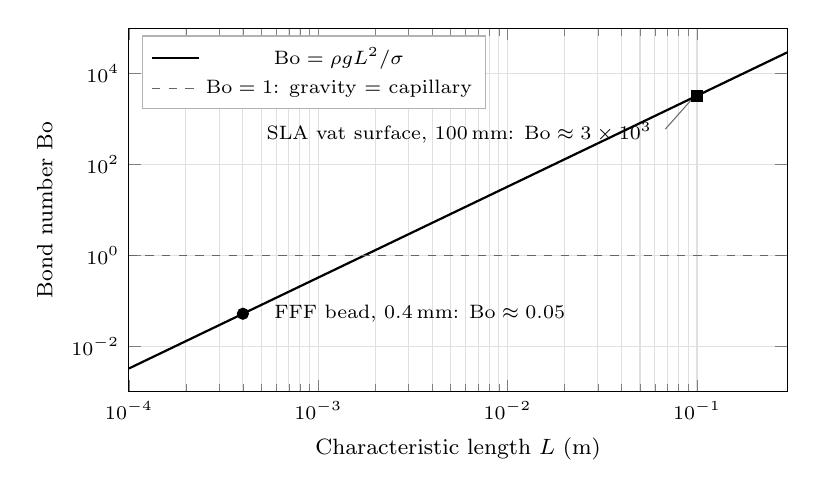
\begin{tikzpicture}
\begin{loglogaxis}[
  width=0.82\textwidth, height=6.2cm,
  xlabel={Characteristic length \(L\) (m)},
  ylabel={Bond number \(\mathrm{Bo}\)},
  xmin=1e-4, xmax=3e-1, ymin=1e-3, ymax=1e5,
  grid=both, grid style={black!12},
  label style={font=\footnotesize},
  tick label style={font=\scriptsize},
  legend style={font=\scriptsize, at={(0.02,0.98)}, anchor=north west,
                draw=black!30},
]
% Bo = rho g L^2 / sigma, with rho=1000, g=9.81, sigma=0.03
\addplot[domain=1e-4:3e-1, samples=80, thick, black]
        {327000*x^2};
\addlegendentry{\(\mathrm{Bo}=\rho g L^{2}/\sigma\)}
% Bo = 1 threshold
\addplot[domain=1e-4:3e-1, samples=2, dashed, black!60] {1};
\addlegendentry{\(\mathrm{Bo}=1\): gravity \(=\) capillary}
% markers
\addplot[only marks, mark=*, mark size=2pt, black]
        coordinates {(4e-4, 0.0523)};
\addplot[only marks, mark=square*, mark size=2pt, black]
        coordinates {(1e-1, 3270)};
\node[font=\scriptsize, anchor=west] at (axis cs:5.2e-4, 0.0523)
     {FFF bead, \(\SI{0.4}{\milli\metre}\): \(\mathrm{Bo}\approx0.05\)};
\node[font=\scriptsize, anchor=east] at (axis cs:6.5e-2, 500)
     {SLA vat surface, \(\SI{100}{\milli\metre}\): \(\mathrm{Bo}\approx3\times10^{3}\)};
\draw[black!55, thin] (axis cs:6.8e-2,600) -- (axis cs:9.3e-2,2600);
\end{loglogaxis}
\end{tikzpicture}
\caption{How much gravity matters, as a function of size, for molten plastic
(\(\rho=\SI{1000}{\kilogram\per\metre\cubed}\),
\(\sigma=\SI{0.03}{\newton\per\metre}\)). Below the dashed line, surface tension
wins and gravity is negligible. A printed bead sits well below it even on Earth,
which is why extrusion still works in orbit. The open surface of a resin tank sits
far above it, which is why resin printers do not.}
\label{fig:bond}
\end{figure}

Experiment supports this reasoning. NASA compared parts printed on the ISS with identical parts printed on the ground
and did find differences in density and strength. When they investigated, the
cause turned out to be a small difference in machine settings --- the gap between
the nozzle and the print bed --- and not microgravity affecting the printing
process \cite{prater2019zerog}. \textbf{This result is what makes the present
proposal possible: it means the process can be developed on the ground, so long as
machine settings are controlled and recorded just as carefully.}

\subsection{Why the alternative processes do not transfer}

The question here is not which printing process makes the best parts, but which
ones still work at all once gravity is gone. Table~\ref{tab:processes} is
therefore arranged by what breaks, not by part quality. In every case that fails,
the reason is the same: the process uses gravity to \emph{put material where it
belongs} --- to settle a flat layer of powder, to hold a level pool of liquid
resin, to drop a droplet onto a target. No amount of tuning replaces that.
Extrusion is the exception, because it places material mechanically and holds it
there with surface tension and viscosity, neither of which cares about
gravity.

\begin{table}[htbp]
\centering
\caption{Which 3D printing processes still work without gravity.}
\label{tab:processes}
\small
\begin{tabularx}{\textwidth}{@{}L{3.1cm} L{2.5cm} X@{}}
\toprule
\textbf{Process family} & \textbf{Viability} & \textbf{Governing reason} \\
\midrule
Material extrusion (FFF) & Demonstrated &
Melt confined and mechanically driven; capillary-dominated bead formation;
adhesion by thermal fusion. Flight heritage since 2014
\cite{prater2019zerog,issnl_amf}. \\
Powder bed fusion (SLS, L-PBF) & Not viable near-term &
Requires a gravity-settled powder layer spread by a recoater. Loose powder
disperses in free fall and constitutes an inhalation, contamination and
electrical hazard in a pressurised volume. \\
Vat photopolymerisation (SLA) & Conditionally viable &
Requires a flat free liquid surface, which does not form in microgravity;
demands a constrained or membrane-bottomed vat and resin containment. \\
Binder jetting & Not viable near-term &
Combines the powder-bed problem with unassisted droplet placement. \\
Directed energy deposition, wire-fed & Demonstrated, high cost &
Wire is mechanically fed and the melt pool retained by surface tension; ESA
demonstrated metal printing aboard the ISS in 2024 \cite{esa_metal3d}. High
power, high thermal load and spatter containment place it beyond an
undergraduate project. \\
Bioprinting & Benefits from microgravity &
Absence of gravitational collapse removes the need for scaffolding; outside the
scope of this proposal. \\
\bottomrule
\end{tabularx}
\end{table}

Material extrusion is therefore selected: it is the only family that is
simultaneously flight-proven, free of loose particulate, modest in power demand,
and benign in its failure modes \cite{asme2023review,technologies2026review}.

\subsection{What must nevertheless change in the machine}

The fact that the \emph{printing physics} survives free fall does not make a lab
printer a space printer. The Department's existing machines cannot be modified,
and in any case a commercial printer is the wrong starting point: its frame,
airflow and control electronics are all designed around assumptions that this
project needs to break. The machine will therefore be designed and built from
components. That is more work, but it buys the freedom to put sensors where they
are needed, to seal and instrument the chamber properly, and --- most importantly
--- to let the SoC drive the motion hardware directly rather than through a
closed commercial controller. The following changes are what the custom build is
for, and they constitute the mechanical work of this project.

\begin{enumerate}[leftmargin=*]
  \item \textbf{Cooling without air.} On Earth, hot air rises and carries heat
        away on its own. In free fall it does not rise at all, so that mechanism
        disappears; and on an unpressurised platform there is no air to move in
        the first place. Heat must then leave by conduction and radiation alone.
        How fast a bead cools decides how well it bonds to the layer below and
        how much stress is locked into the part, so this is not a detail --- it
        changes the thermal design of the whole machine. Section~\ref{sec:thermal}
        sets out how it is handled here.
  \item \textbf{Containing what the plastic gives off.} Melting plastic releases
        fumes and very fine particles. In a pressurised cabin that is a
        crew-health problem; in vacuum it becomes a molecular contamination
        problem, which is why outgassing is a standard space-materials screening
        requirement. Either way the chamber must be closed and the emissions
        captured or pumped away.
  \item \textbf{Everything must be held down deliberately.} Nothing stays put
        under its own weight. The part must be gripped to the bed, released in a
        controlled way, and caught once released, and any debris must be
        captured --- otherwise it simply floats away.
  \item \textbf{Motors have to sit outside the chamber.} This one bites
        immediately. Stepper motors are cooled almost entirely by convection
        into the surrounding air; remove it and heat leaves only by conduction
        through the mounting face, so continuous torque must be derated
        substantially --- suppliers of vacuum-rated motors quote reductions of
        \SIrange{20}{50}{\percent} and sometimes a factor of several, depending
        on duty cycle and mounting. Vacuum-rated motors exist but are expensive.
        The design instead keeps the motors outside the vacuum boundary and
        drives the mechanism through the wall. CoreXY makes this natural: both
        \(X\) and \(Y\) motors are frame-mounted and stationary by construction,
        so only belts cross the boundary. It does, however, argue for a Bowden
        extruder rather than direct drive, since direct drive would put a motor
        on the moving carriage inside the chamber.
  \item \textbf{A controlled filament path.} On Earth the spool stays neat and
        the filament stays taut partly because of gravity. In orbit it will not,
        so the feed needs active tension control and a sensor to detect the
        filament slipping.
  \item \textbf{It has to survive the launch.} The machine will be shaken far
        harder on the way up than any lab instrument ever is, which changes how
        stiff the frame must be and how everything is fastened.
\end{enumerate}

\subsection{Thermal control without air}
\label{sec:thermal}

Blowing air across the part is how every desktop printer manages cooling, and it
is the wrong answer here. It is worth being precise about why, because fans are
not universally wrong in space: inside a pressurised module there is cabin air,
forced convection works, and it is the standard flight-proven solution --- the
printers currently aboard the ISS rely on it. But this project's stated target is
the case where crew are absent: a free-flying platform, an external payload, or a
lunar surface asset. There, either there is no air at all, or the volume is small
and sealed and a fan is simply recirculating its own contamination. A fan also
has bearings, which is a wear item in a machine whose entire premise is
unattended operation for weeks, and it injects broadband vibration and airflow
noise into exactly the accelerometer and acoustic channels this project uses to
detect nozzle clogs.

The machine is therefore designed around conduction and radiation, and the
chamber is built to be evacuated rather than ventilated.

\paragraph{Radiation is not negligible at extrusion temperatures.} It is easy to
dismiss radiative cooling as a small effect, but the fourth-power dependence
rescues it. For a freshly deposited bead at \(\SI{240}{\celsius}\)
(\(\SI{513}{\kelvin}\)) radiating to chamber walls held at
\(\SI{60}{\celsius}\), with emissivity \(\varepsilon \approx 0.9\),

\begin{equation}
  q'' = \varepsilon\sigma\left(T_\text{bead}^{4}-T_\text{wall}^{4}\right)
      \approx 0.9 \times \num{5.67e-8}\left(513^{4}-333^{4}\right)
      \approx \SI{2.9}{\kilo\watt\per\metre\squared}.
\end{equation}

That is a real heat flux, and it is controllable: chamber wall temperature and
wall emissivity become design variables, and the same equation says that a
\(\SI{20}{\celsius}\) change in wall temperature is a usable control input.

\paragraph{The thermal architecture.}
\begin{itemize}
  \item \textbf{Hot end:} heat is conducted off the heat break rather than blown
        off it. The published vacuum-FFF systems use a pumped liquid cold end
        \cite{scirep2025vacuumfff,peek_vacuum2025}, and that remains the
        fallback, but the preferred solution here is a sintered-wick heat pipe.
        Heat pipes are capillary-driven, contain no pump, and are entirely
        gravity-independent --- which is why they are standard on spacecraft, and
        why they suit a machine intended to run unattended for weeks. Removing
        the pump removes the last rotating part in the thermal path.
  \item \textbf{Part cooling:} conduction down through the deposited layers into
        a temperature-controlled build plate, plus radiation to the chamber
        walls. There is no impingement cooling on the bead.
  \item \textbf{Chamber walls:} held at a commanded temperature by resistive
        film heaters under closed-loop control. Thermoelectric modules were
        considered and rejected: for ABS and polycarbonate the chamber wants to
        be \emph{hot} --- around \SI{60}{\celsius}, to stop the part warping ---
        so the cooling direction would essentially never be used, and a
        thermoelectric stage would draw over \SI{100}{\watt} to do what a film
        heater does for a fraction of it. Heat leaves the chamber passively to
        the laboratory through the wall.
  \item \textbf{Layer time as the primary cooling control.} This is the
        consequence that matters for the control problem. Without convection,
        the fastest available cooling mechanism is gone, so interlayer
        temperature is regulated by \emph{how long the machine waits} --- dwell
        time, layer scheduling, and toolpath ordering --- rather than by how hard
        a fan blows. Thermal management moves from the actuator domain into the
        planner, which makes it a scheduling problem for the controller running
        on the SoC.
\end{itemize}

\paragraph{How much vacuum is actually required.} It is worth deriving this
rather than assuming, because the answer sets the single largest item in the
budget. Buoyancy-driven convection is governed by the Rayleigh number,

\begin{equation}
  \mathrm{Ra} \;=\; \frac{\rho^{2}g\beta\,\Delta T\,L^{3}c_p}{\mu k},
\end{equation}

and the relevant feature is the \(\rho^{2}\) dependence: halving the gas density
quarters the tendency to convect. For this chamber
(\(L \approx \SI{0.15}{\metre}\), \(\Delta T \approx \SI{180}{\kelvin}\) between
a \(\SI{240}{\celsius}\) bead and \(\SI{60}{\celsius}\) walls) the Rayleigh
number at atmospheric pressure is of order \num{e7}. Convective cells do not form
below \(\mathrm{Ra} \approx \num{e3}\), so a reduction of about four orders of
magnitude is required, which corresponds to a hundredfold fall in density ---
roughly \SI{10}{\milli\bar}.

\textbf{The chamber is therefore specified at \SI{1}{\milli\bar}}, which carries
an order of magnitude of margin over the requirement.

One limitation should be stated rather than glossed over. Suppressing
\emph{convection} is not the same as removing the gas. At \SI{1}{\milli\bar} the
mean free path in air is around \SI{65}{\micro\metre}, still short compared with
millimetre-scale gaps, so residual gas \emph{conduction} persists; it falls away
only below roughly \SI{0.1}{\milli\bar}. The chamber therefore reproduces the
absence of buoyancy-driven convection exactly --- which is the microgravity
condition, and is what the ISS printers use fans to compensate for --- while only
partially reproducing the conduction environment of an unpressurised platform.
The pressure sweep of Section~3.5 maps both regimes, and the distinction is
recorded here rather than discovered in review. This matters practically:
\SI{1}{\milli\bar} is reached by a single-stage rotary-vane pump costing a
fraction of the two-stage pump needed for \(\SI{e-3}{\milli\bar}\), and it needs
only a simple analogue gauge rather than a Pirani head. The published vacuum-FFF
work operates far lower --- down to \(\SI{e-4}{\milli\bar}\)
\cite{scirep2025vacuumfff} --- but those experiments are also characterising
outgassing and contamination, which this project is not. Specifying more vacuum
than the physics requires would consume roughly a fifth of the total budget for
no experimental gain.

\paragraph{Borrowed directly from spacecraft thermal practice.} None of this
needs inventing. Satellites have solved the no-convection problem for sixty
years, and the following are cheap, available, and directly applicable:

\begin{itemize}
  \item \textbf{Controlled surface emissivity.} Emissivity appears explicitly in
        the radiative flux above, so it is a design variable rather than a
        material accident. High-emissivity coating on the chamber interior
        maximises heat absorbed from the part; polished surfaces isolate what
        should stay hot. It also becomes a cheap experimental variable: sweeping
        wall emissivity and measuring the resulting cooling rate is a direct
        check on the ANSYS radiation model.
  \item \textbf{Flexible thermal straps.} Braided copper is the standard
        spacecraft answer for conducting heat across a joint that has to move.
  \item \textbf{Multi-layer insulation.} Aluminised film around the hot end and
        chamber exterior. Worth noting that MLI only works properly \emph{in
        vacuum} --- in air the trapped gas conducts straight through it --- so
        this is one of the few benchtop machines where it earns its place.
  \item \textbf{Isolation standoffs.} Low-conductivity mounts (G10 or PEEK) to
        stop heat leaking into the frame, where it would distort the structure
        and detune the sensors.
  \item \textbf{Heaters, not just cooling.} Most spacecraft thermal control is
        about keeping things warm. The same applies here: with convection gone
        and walls held cold for part cooling, the chamber will need trim heating
        to hold the filament path and sensors in range.
\end{itemize}

\paragraph{The problem this creates: the hot end moves.} On Earth this is
invisible, because the cooling fan simply rides on the carriage. Conducting heat
off a moving gantry is harder, and there are only three ways to do it --- braid,
a heat pipe with a compliant section, or fluid tubing with a service loop. Each
trades thermal conductance against the drag force it adds to the motion system,
and that drag directly affects positioning accuracy and therefore the quality of
the layer imagery the whole inspection loop depends on. This is a real trade
rather than a detail, and it is resolved as an explicit task in WP3
(Table~\ref{tab:strap}).

\paragraph{This is established, not speculative.} FFF has been demonstrated at
\(\SI{e-4}{\milli\bar}\), where convective heat transfer is negligible, using
active water cooling to keep components from overheating
\cite{scirep2025vacuumfff}. Polycarbonate has been printed under low vacuum with
no loss of mechanical performance and with contamination low enough to
characterise \cite{ceas2021lowvacuum}. High-temperature space-relevant polymers
--- PEKK, PEI and their carbon-nanotube composites --- have been printed in high
vacuum \cite{jsr2023vacuumfff}, and for PEEK, layer adhesion actually
\emph{improves} as pressure falls \cite{peek_vacuum2025}. That last group also
report that low-cost vacuum equipment is sufficient, which is what makes this
approach viable on an undergraduate budget.

\paragraph{One finding worth flagging in advance.} The vacuum FFF work reports
that the hot-end PID parameters had to be retuned substantially for vacuum
operation, because the heat-loss path changes completely
\cite{scirep2025vacuumfff}. That is a control-design problem, it lands squarely
in the MATLAB work of Section~\ref{sec:tools}, and it is a small original
contribution available cheaply: nobody has characterised how a
\emph{closed-loop, sensor-driven} thermal controller must change when convection
is removed.

\subsection{Establishing microgravity representativeness without flight access}

Gravity cannot be switched off on a bench, but its two consequences can be
attacked separately, and the evacuable chamber does most of the work.

\emph{Removing convection is not an approximation --- it is exact.} As shown in
Section~\ref{sec:thermal}, the Rayleigh number falls as \(\rho^{2}\), so a
chamber held at \SI{1}{\milli\bar} suppresses convection with an order of
magnitude of margin. A ground chamber at low pressure therefore reproduces the
\emph{thermal} environment of free fall faithfully rather than approximating it,
and reproduces an unpressurised orbital platform exactly. Chamber pressure
becomes an experimental variable in its own right: printing the same specimen at
a sequence of pressures from ambient down to \SI{1}{\milli\bar} maps where
convection ceases to matter and gives a direct experimental check on the ANSYS
zero-gravity thermal model rather than leaving it unvalidated. The predicted
transition near \SI{10}{\milli\bar} is itself a falsifiable claim, which is
better than an assumption.

\emph{Removing the body force on the melt} is the part that cannot be reproduced
on the ground, so it is addressed by argument and by \emph{orientation testing}:
print the same specimen with the machine on its side and inverted. If results do
not change when gravity points elsewhere, they are unlikely to change when it is
absent --- and Section~\ref{sec:bond} already shows why this should be expected
at the bead scale. Alongside this, all comparison specimens are printed from one
filament batch with identical recorded settings, following NASA's method
\cite{prater2019zerog}.

Between them these cover the two mechanisms, and the pressure sweep is the
stronger of the two because it is a measurement rather than an inference. It is
also worth being clear about what the chamber is: a \emph{simulator}, not a
prototype subsystem. Its purpose is to reproduce on a bench the pressure that an
unpressurised orbital platform provides at no cost, so the pressure sweep is a
ground-only diagnostic that validates the thermal model. A flight unit would
simply operate at the low end of that sweep permanently
(Section~\ref{sec:power}). A
parabolic flight would still add value, but it is follow-on work and nothing here
depends on it.

%=======================================================================
\section{Research Gap}
%=======================================================================

I surveyed three separate research fields. Each one is well developed on its own,
but the place where they meet has not been studied (Table~\ref{tab:gap}). Each
field, it turns out, assumes away exactly the problem that one of the others
works on.

\begin{figure}[htbp]
\centering
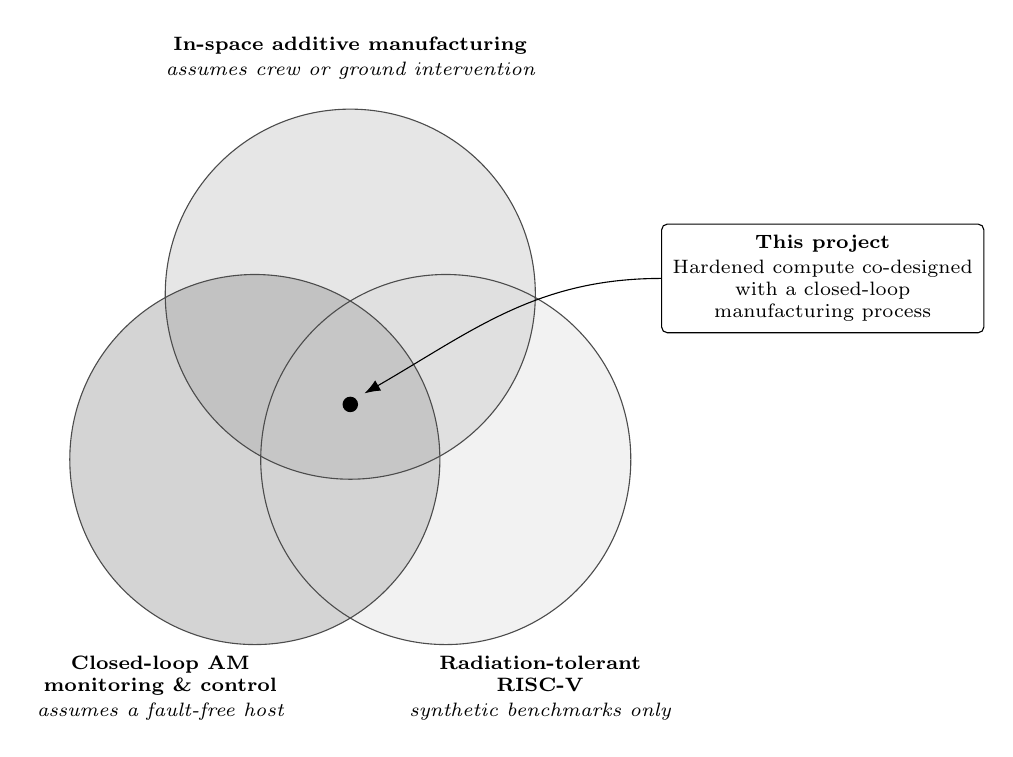
\begin{tikzpicture}[font=\footnotesize]
  \def\rr{2.35}
  \coordinate (A) at (90:1.40);
  \coordinate (B) at (210:1.40);
  \coordinate (C) at (330:1.40);
  \begin{scope}[opacity=0.28]
    \fill[black!35] (A) circle (\rr);
    \fill[black!60] (B) circle (\rr);
    \fill[black!18] (C) circle (\rr);
  \end{scope}
  \draw[black!70] (A) circle (\rr);
  \draw[black!70] (B) circle (\rr);
  \draw[black!70] (C) circle (\rr);

  % --- labels placed outside the circles ---
  \node[align=center, font=\scriptsize] at ($(A)+(0,3.0)$)
       {\textbf{In-space additive manufacturing}\\[1pt]
        \itshape assumes crew or ground intervention};

  \node[align=center, font=\scriptsize] at ($(B)+(-1.20,-2.90)$)
       {\textbf{Closed-loop AM}\\\textbf{monitoring \& control}\\[1pt]
        \itshape assumes a fault-free host};

  \node[align=center, font=\scriptsize] at ($(C)+(1.20,-2.90)$)
       {\textbf{Radiation-tolerant}\\\textbf{RISC-V}\\[1pt]
        \itshape synthetic benchmarks only};

  % --- the gap ---
  \fill[black] (0,0) circle (2.8pt);
  \node[draw, fill=white, rounded corners=2pt, align=center,
        font=\scriptsize, inner sep=4pt] (gapbox) at (6.0,1.6)
       {\textbf{This project}\\[1pt]
        Hardened compute co-designed\\with a closed-loop\\manufacturing process};
  \draw[ar] (gapbox.west) to[out=180,in=30] (0.18,0.14);
\end{tikzpicture}
\caption{The three fields this project draws on, and the gap where they meet.
Each field is mature on its own, and each takes for granted the very thing the
next one studies.}
\label{fig:venn}
\end{figure}

\begin{table}[htbp]
\centering
\caption{Maturity and assumptions of the three contributing literatures.}
\label{tab:gap}
\small
\begin{tabularx}{\textwidth}{@{}L{3.0cm} X X@{}}
\toprule
\textbf{Literature} & \textbf{Mature in} & \textbf{Assumes away} \\
\midrule
In-space additive manufacturing &
Process feasibility in microgravity; material characterisation; flight heritage
\cite{prater2019zerog,asme2023review,technologies2026review} &
Autonomy: presumes crew or ground intervention \\[2pt]
Closed-loop AM monitoring and control &
Optical, thermal, acoustic and vibration sensing; CNN and SVM defect classifiers
reporting \SIrange{90}{95}{\percent} accuracy; autonomous parameter correction
\cite{fff_monitoring_review,saluja2020warping,cirp2024closedloop,anomaly_fff_ml2023} &
Computing platform reliability: presumes a desktop-class, fault-free host \\[2pt]
Radiation-tolerant RISC-V &
TMR, ECC, lockstep, scrubbing, fault awareness; beam-validated cross-sections
\cite{wilson2019neutron,electronics2023faultawareness,noelv_proton,trikarenos2023} &
Workload realism: benchmarked on CoreMark, Embench and Dhrystone; no real-time
control or ML inference under fault \\
\bottomrule
\end{tabularx}
\end{table}

\paragraph{Gap 1: the test programs are not realistic.}
The cost of protecting a processor is always measured while it runs a benchmark
program. A printer controller behaves nothing like a benchmark. It has to respond
within fixed deadlines, it reads sensors continuously, and it runs a neural
network in the middle of the control loop. Losing \SI{27}{\percent} of the clock
speed barely matters to a benchmark, which simply finishes later. For a motion
controller, the same slowdown may mean a deadline is missed and the machine
misbehaves. Nobody has measured the cost of protection while running a real
manufacturing control workload.

\paragraph{Gap 2: the inspection step can fail silently.}
A self-correcting printer acts on whatever its defect classifier reports. If
radiation flips a bit inside that neural network --- in one of its weights, in an
intermediate value, or in the threshold it compares against --- the program does
not crash and no error is reported. It simply gives the wrong answer, with full
confidence. The printer then ``fixes'' a defect that was never there, or ignores a
real one. Error-correcting memory protects stored data, but nobody has measured
how often a bit flip changes the final decision a printer acts on, or tested what
kind of redundancy protects that particular step.

\begin{figure}[htbp]
\centering
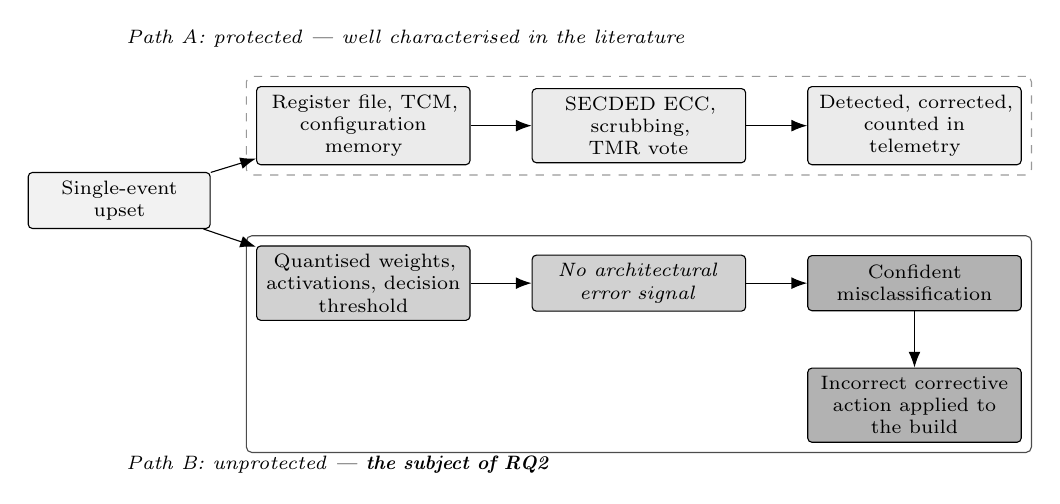
\begin{tikzpicture}[font=\scriptsize, node distance=4mm]

% --- protected path (upper) ---
\node[blk, fill=black!5, text width=21mm] (strike) at (0,0)
     {Single-event\\upset};
\node[blk, fill=black!8, text width=25mm] (mem) at (3.1,0.95)
     {Register file, TCM,\\configuration memory};
\node[blk, fill=black!8, text width=25mm] (ecc) at (6.6,0.95)
     {SECDED ECC,\\scrubbing, TMR vote};
\node[blk, fill=black!8, text width=25mm] (ok) at (10.1,0.95)
     {Detected, corrected,\\counted in telemetry};

% --- unprotected path (lower) ---
\node[blk, fill=black!18, text width=25mm] (inf) at (3.1,-1.05)
     {Quantised weights,\\activations, decision\\threshold};
\node[blk, fill=black!18, text width=25mm] (nosig) at (6.6,-1.05)
     {\emph{No architectural}\\\emph{error signal}};
\node[blk, fill=black!30, text width=25mm] (wrong) at (10.1,-1.05)
     {Confident\\misclassification};
\node[blk, fill=black!30, text width=25mm] (act) at (10.1,-2.6)
     {Incorrect corrective\\action applied to\\the build};

\draw[ar] (strike) -- (mem);
\draw[ar] (strike) -- (inf);
\draw[ar] (mem) -- (ecc);
\draw[ar] (ecc) -- (ok);
\draw[ar] (inf) -- (nosig);
\draw[ar] (nosig) -- (wrong);
\draw[ar] (wrong) -- (act);

\node[lbl, anchor=west] at (0.05,2.05) {Path A: protected --- well characterised in the literature};
\node[lbl, anchor=west] at (0.05,-3.35) {Path B: unprotected --- \textbf{the subject of RQ2}};

\begin{scope}[on background layer]
  \node[fit=(mem)(ok), draw=black!40, dashed, rounded corners=2pt,
        inner sep=3.5pt] {};
  \node[fit=(inf)(wrong)(act), draw=black!70, rounded corners=2pt,
        inner sep=3.5pt] {};
\end{scope}
\end{tikzpicture}
\caption{What happens when radiation flips a bit inside the printer's
controller. If the bit is in memory or control logic (Path~A), existing
protection catches it, fixes it, and records it. If it is inside the neural
network (Path~B), nothing catches it: the program does not crash, it just returns
a wrong answer confidently, and the printer then acts on that wrong answer. How
often this happens has never been measured.}
\label{fig:faultpath}
\end{figure}

\paragraph{Gap 3: nothing tells the two kinds of fault apart.}
Faults in the computer and faults in the printer are handled by completely
separate machinery, and neither knows about the other. The trouble is that they
look identical from outside. A jammed extruder and a crashed control program both
show up as ``no plastic is coming out''. If the machine guesses wrong about which
one it is, it applies the wrong fix --- resetting the processor will not clear a
jam. No published design reasons about both kinds of fault together.

\medskip\noindent
These three questions are genuinely open, and answering them needs about
\rupee\,67{,}200 of equipment. Problems that are both unsolved and cheap to attack are rare,
which is why I am proposing this rather than a more conventional VLSI topic.

%=======================================================================
\section{Research Questions and Hypotheses}
%=======================================================================

\begin{description}[leftmargin=1.5cm,style=nextline,font=\bfseries]

\item[RQ1.] Which combination of protection techniques gives the most
reliability per unit of chip area and speed, for a small RISC-V processor running
a real 3D printing control workload?

\emph{H1.} Protecting only the parts that matter most --- triplicating the
control logic and status registers, using error-correcting memory, and running two
cores in step to check each other, while leaving the arithmetic unit unprotected
--- will get within \SI{20}{\percent} of the reliability of triplicating
everything, at less than half the cost in chip area, and will still meet the
timing deadlines that full triplication would break.

\item[RQ2.] When radiation flips a bit inside the neural network that inspects
each layer, what happens, and how often does the printer end up making the wrong
decision as a result?

\emph{H2.} A significant share of bit flips in the neural network will produce a
wrong answer with no error reported at all, and that share will be larger than the
share that produces a visible crash. If so, the inspection step will turn out to
cause more bad decisions than any other part of the system, even though it is the
smallest part of it.

\item[RQ3.] Can one system reliably tell a computer fault from a printer fault
and apply the right fix to each, and how accurately?

\emph{H3.} Combining two sources of evidence --- the error counters inside the
processor and the physical sensor readings from the printer --- will tell the two
kinds of fault apart far better than either source can on its own.

\end{description}

RQ1 and RQ2 are what I commit to answering in twelve months. RQ3 will be attempted
if there is time; if not, it is the obvious next step.

%=======================================================================
\section{Objectives}
%=======================================================================

The objectives below turn the research questions of Section~5 into concrete things
that can be built and checked. Each one has a clear pass or fail test, so progress
at the review meetings in Section~8 can be judged on evidence rather than
opinion.

The \textbf{Core} objectives are what I commit to in twelve months, and together
they answer RQ1 and RQ2. The \textbf{Extension} objective answers RQ3 and will
only be attempted if the core work finishes early. I have listed it rather than
leaving it out, because you should be able to see where the project leads before
agreeing to its first year.

O1 and O2 are the hardware; O3 and O4 are the printer and its control loop; O5 and
O6 are the experiment itself. O1 is checked at month~2 (Section~\ref{sec:prep}), and that is
the one point at which the project should be stopped if it is not working.

\begin{table}[htbp]
\centering
\caption{Project objectives and success criteria.}
\label{tab:objectives}
\small
\begin{tabularx}{\textwidth}{@{}c L{5.0cm} X c@{}}
\toprule
\textbf{\#} & \textbf{Objective} & \textbf{Success criterion} & \textbf{Tier} \\
\midrule
O1 & Establish a verified RISC-V SoC baseline on FPGA &
Boots an RTOS; passes the \texttt{riscv-arch-test} compliance suite via RISCOF;
continuous-integration pipeline operational; bus adapter defined so that the
core remains replaceable & Core \\
O2 & Implement a parameterised hardening architecture (ECC, selective TMR,
DCLS, scrubbing, watchdog escalation, error counters) &
All mitigations independently enabled or disabled at build time, permitting
controlled comparison & Core \\
O3 & Design, analyse and build a microgravity-representative FFF machine &
CAD model and ANSYS structural and thermal analysis complete; machine built and
printing repeatably; evacuable chamber with conduction and radiation thermal
control; optical, thermal, vibration and feed sensing & Core \\
O4 & Implement closed-loop defect detection and autonomous correction &
\(\geq 4\) defect classes detected; \(\geq \SI{90}{\percent}\) classification
accuracy after quantisation; corrective actions bounded by a hardware safety
envelope & Core \\
O5 & Develop an open fault-injection framework &
Injects SEU and multiple-bit upsets into RTL simulation and FPGA
configuration and user memory; injects physical process faults reproducibly &
Core \\
O6 & Execute the characterisation campaign; answer RQ1 and RQ2 &
Statistically adequate sample sizes with reported confidence intervals & Core \\
O7 & Address RQ3: unified compute/process fault discrimination &
Discrimination accuracy quantified against single-modality baselines &
Extension \\
O8 & Disseminate &
Two submitted papers; open-source RTL, framework and dataset & Core \\
\bottomrule
\end{tabularx}
\end{table}

%=======================================================================
\section{Methodology}
%=======================================================================

\subsection{Overall approach}

The hardware will be developed using the European Space Agency's standard process
for FPGA and chip design, ECSS-E-ST-20-40C, together with its quality companion
ECSS-Q-ST-60-03C \cite{ecss2040c,ecssq6003c}. The choice of protection techniques
follows the ESA handbook on radiation effects \cite{ecsshb2040a}. Measurements
follow ordinary controlled-experiment practice: change one thing at a time and
compare against a fixed baseline.

Following a recognised space standard from day one is deliberate. It costs very
little extra now, while the project is small. Adding it later, once the design
already exists, is painful --- and without it, a design can never be put forward
for a real flight, however good it is.

\begin{figure}[htbp]
\centering
\resizebox{\textwidth}{!}{%
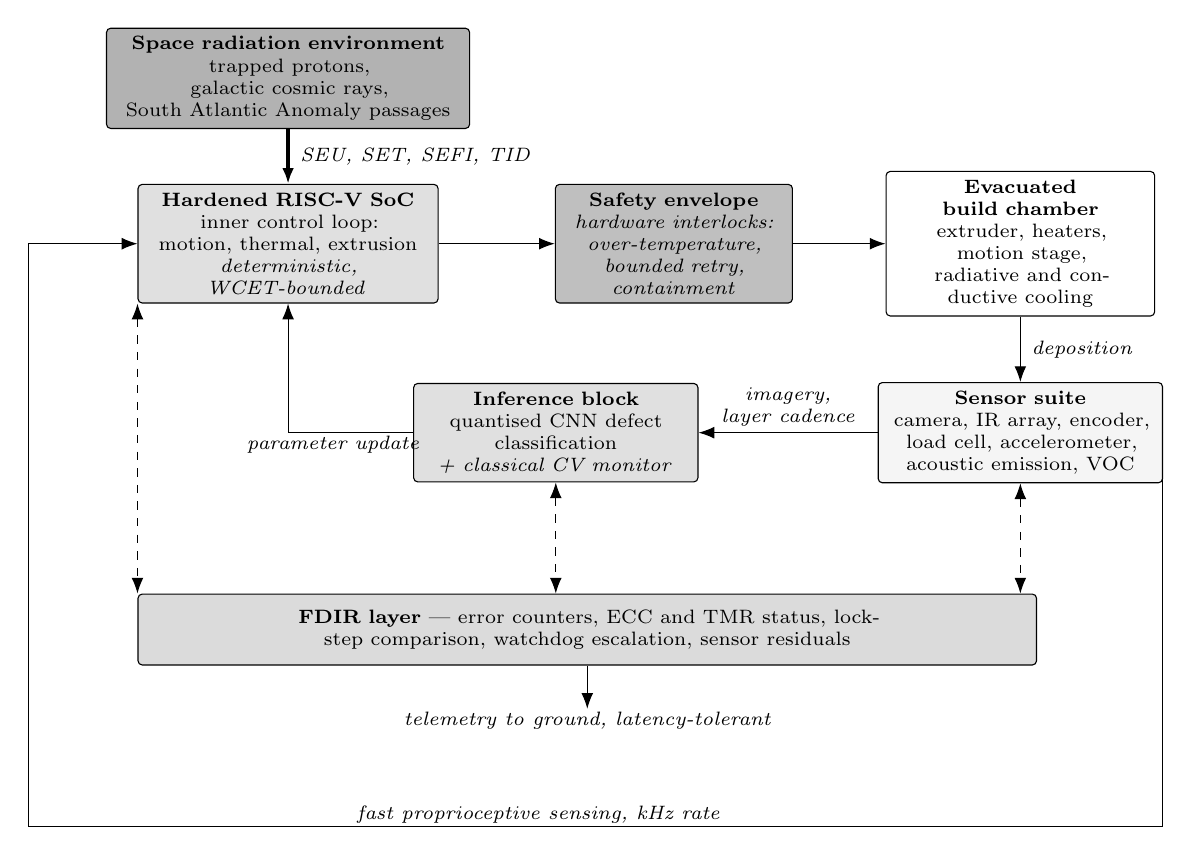
\begin{tikzpicture}[font=\scriptsize]

% --- environment ---
\node[blk, fill=black!30, text width=44mm] (rad) at (2.5,3.1)
     {\textbf{Space radiation environment}\\
      trapped protons, galactic cosmic rays,\\
      South Atlantic Anomaly passages};

% --- forward path ---
\node[hard, text width=36mm] (soc) at (2.5,1.0)
     {\textbf{Hardened RISC-V SoC}\\
      inner control loop:\\motion, thermal, extrusion\\
      \itshape deterministic, WCET-bounded};

\node[danger, text width=28mm] (safe) at (7.4,1.0)
     {\textbf{Safety envelope}\\
      \itshape hardware interlocks:\\
      \itshape over-temperature,\\\itshape bounded retry,\\
      \itshape containment};

\node[soft, text width=32mm] (printer) at (11.8,1.0)
     {\textbf{Evacuated build chamber}\\
      extruder, heaters, motion stage,\\
      radiative and conductive cooling};

% --- return path ---
\node[sens, text width=34mm] (sensors) at (11.8,-1.4)
     {\textbf{Sensor suite}\\
      camera, IR array, encoder,\\
      load cell, accelerometer,\\
      acoustic emission, VOC};

\node[hard, text width=34mm] (infer) at (5.9,-1.4)
     {\textbf{Inference block}\\
      quantised CNN defect\\classification\\
      \itshape + classical CV monitor};

% --- FDIR band ---
\node[blk, fill=black!14, text width=112mm, minimum height=9mm] (fdir) at (6.3,-3.9)
     {\textbf{FDIR layer} --- error counters, ECC and TMR status, lockstep comparison,
      watchdog escalation, sensor residuals};

% --- arrows ---
\draw[ar, very thick] (rad) -- node[lbl, right, xshift=1mm]
     {SEU, SET, SEFI, TID} (soc);
\draw[ar] (soc) -- (safe);
\draw[ar] (safe) -- (printer);
\draw[ar] (printer) -- node[lbl, right, xshift=1mm] {deposition} (sensors);
\draw[ar] (sensors) -- node[lbl, above, align=center, yshift=0.4mm]
     {imagery,\\layer cadence} (infer);
\draw[ar] (infer.west) -| node[lbl, below, pos=0.32]
     {parameter update} (soc.south);

% fast sensing path, routed outside everything
\draw[ar] (sensors.east) -- (13.6,-1.4) -- (13.6,-6.4) --
          node[lbl, above, pos=0.55] {fast proprioceptive sensing, kHz rate}
          (-0.8,-6.4) -- (-0.8,1.0) -- (soc.west);

% FDIR monitors
\draw[arr, dashed] (soc.south west) -- (soc.south west |- fdir.north);
\draw[arr, dashed] (infer.south) -- (infer.south |- fdir.north);
\draw[arr, dashed] (sensors.south) -- (sensors.south |- fdir.north);
\draw[ar] (fdir.south) -- ++(0,-0.55)
     node[below, lbl] {telemetry to ground, latency-tolerant};
\end{tikzpicture}}
\caption{End-to-end system pipeline. Radiation acts on the controller, not on
the process: charged particles upset the SoC, whose corrupted output then
propagates forward through the safety envelope into the physical build, and
returns through the sensor suite. Two return paths operate at different rates
--- fast proprioceptive sensing closes the inner control loop, while imagery
closes the slower inspection loop through the inference block. The FDIR layer
observes all three stages, which is what makes fault-origin discrimination
(RQ3) possible at all.}
\label{fig:pipeline}
\end{figure}

\subsection{Design and analysis tools}
\label{sec:tools}

The work spans four domains, and each is handled with the standard tool for it
rather than with improvised alternatives.

\begin{itemize}
  \item \textbf{SolidWorks --- mechanical design.} The full printer, chamber,
        filament path and sensor mounts are modelled in CAD before anything is
        cut. This produces the fabrication drawings, the bill of materials, and
        the geometry that feeds directly into the analysis below.
  \item \textbf{ANSYS --- structural and thermal analysis.} Two uses. Structural:
        modal and random-vibration analysis of the frame and chamber, so that the
        design can be assessed against launch-representative loads by analysis
        even though no shaker test is planned within the twelve months.
        \emph{Thermal: this is where the microgravity argument becomes a design
        calculation rather than a claim.} The chamber is modelled in three
        configurations --- at \(1\,g\) and atmospheric pressure, with the
        gravitational body force set to zero, and at reduced pressure --- to show
        that the evacuated ground chamber reproduces the free-fall thermal
        environment. Conduction and surface-to-surface radiation are the transport
        mechanisms; there is no convection term to size a fan against. What the
        analysis produces instead is the build-plate power, the chamber wall
        temperature setpoint, the required wall emissivity, the minimum layer dwell
        time needed to reach the target interlayer temperature, and the
        conductance required of the moving thermal link
        (Section~\ref{sec:thermal}).
  \item \textbf{MATLAB and Simulink --- control design.} Plant identification
        from measured step responses, controller design and discretisation for
        the motion, thermal and extrusion loops, stability margins, and
        hardware-in-the-loop testing of the control law before it is committed to
        the SoC. Because the heat-loss path changes completely once convection
        is removed, the thermal loops are identified and tuned separately at
        atmospheric pressure and under vacuum --- published vacuum-FFF work
        reports that hot-end PID parameters differ substantially between the two
        \cite{scirep2025vacuumfff}. The Simulink plant model doubles as the
        reference against which sensor residuals are computed, which is what
        makes the process-fault branch of Figure~\ref{fig:fdir} possible.
  \item \textbf{FPGA and verification toolchain.} AMD Vivado for the SRAM-based
        device and Microchip Libero for the flash-based device; Verilator for
        fast simulation; RISCOF and \texttt{riscv-arch-test} for instruction-set
        compliance; \texttt{riscv-dv} and Spike for randomised
        co-simulation. All of the verification tooling is open-source.
\end{itemize}

Vivado and Libero are free at the editions required. SolidWorks, ANSYS and MATLAB
are already licensed to the Institute for teaching use, so no new software
purchase is requested.

\subsection{WP0 --- Planning (months 1--2)}
\label{sec:prep}

I am entering the third year of the B.E.\ programme and have not yet written
hardware description code at any serious scale. Rather than gloss over that, the
first two months are set aside openly as a learning phase, with specific things to
deliver and a real stop/continue decision at the end of month~2.

\begin{itemize}
  \item \textbf{Weeks 1--4: learn the tools.} SystemVerilog, plus the Verilator
        and Vivado (or Libero) flow. To prove it works, I will build and test two
        small blocks --- an arithmetic unit and a serial port --- with automatic
        tests, and run them on a real board.
  \item \textbf{Weeks 5--8: get a RISC-V processor running.} Put the chosen
        open-source core onto the board, run the official RISC-V test suite
        against it, boot a small real-time operating system, and set up automatic
        testing so every change is checked.
  \item \textbf{Throughout: finish the literature review.} Search IEEE Xplore,
        Scopus, ScienceDirect and NASA's technical reports using a search plan
        fixed in advance, and expand Table~\ref{tab:gap} into a full survey.
\end{itemize}

\textbf{The month~2 decision.} If the processor is not running the test suite on
real hardware by the end of month~2, the project should be cut back or stopped
then --- not at month~10, by which point far more time has been spent. I would
rather this be applied strictly than generously.

\subsection{WP1 --- Build the SoC (months 2--5)}

\paragraph{Base core: Ibex.}
I will not write a processor from scratch. Writing one teaches you a great deal,
but it is not a research result --- hundreds already exist, and mine would be
worse. The new work here is the protection scheme and the measurements, so the
project starts from a proven open-source core.

\textbf{The core is lowRISC's Ibex} \cite{ibex}, a small 32-bit RISC-V CPU used
in OpenTitan. The reason is specific rather than general: Ibex already implements,
as configuration options, most of the protection mechanisms this project sets out
to measure. Turning them on is a parameter; \emph{measuring what they cost, and
what they miss, is the research}. Building them myself would consume the schedule
and produce implementations a reviewer would reasonably distrust.

\begin{table}[htbp]
\centering
\caption{Base core comparison. Ibex is selected; the others remain named
fallbacks.}
\label{tab:cores}
\small
\begin{tabularx}{\textwidth}{@{}L{2.4cm} L{2.2cm} X@{}}
\toprule
\textbf{Core} & \textbf{Language} & \textbf{Assessment} \\
\midrule
\textbf{Ibex}\newline (lowRISC) & SystemVerilog &
\textbf{Selected.} Dual-core lockstep, register-file and cache ECC, hardened PC,
shadow CSRs and alert outputs all exist as parameters
(Table~\ref{tab:secureibex}). Strong CI, riscv-dv and formal verification behind
it. Deployed in OpenTitan, so the implementations are scrutinised. \\
NEORV32 \cite{neorv32} & VHDL &
\emph{Fallback.} Complete SoC rather than a bare core, so bring-up is faster ---
but every protection mechanism would have to be written and then defended.
Reachable in days via the bus adapter (Figure~\ref{fig:adapter}). \\
CV32E40S\newline (OpenHW) & SystemVerilog &
\emph{Fallback.} Safety and security variant with an industrial UVM environment,
but \texttt{core-v-verif} is a large thing to learn alongside everything else. \\
CVA6 \cite{cva6repo} & SystemVerilog &
\emph{Excluded.} Application-class; expects external DRAM, which the Boolean
Board does not have. \\
\bottomrule
\end{tabularx}
\end{table}

\paragraph{What Ibex already provides.}
Setting the \texttt{SecureIbex} parameter enables a set of features developed for
security-critical use, which map almost directly onto radiation-tolerance needs
\cite{ibexsecurity}. Table~\ref{tab:secureibex} lists them alongside the fault
class each addresses.

\begin{table}[htbp]
\centering
\caption{Ibex security features and the radiation fault classes they address.
The rightmost column is the honest accounting of what is adopted versus what
this project contributes.}
\label{tab:secureibex}
\small
\begin{tabularx}{\textwidth}{@{}L{4.0cm} X L{2.3cm}@{}}
\toprule
\textbf{Mechanism} & \textbf{What it catches} & \textbf{Origin} \\
\midrule
Dual-core lockstep & Shadow core runs on delayed inputs; outputs compared
against delayed main-core outputs; mismatch raises a major alert. The delay
\emph{is} temporal diversity, so common-mode transients are caught too & Ibex \\
Register-file ECC and write-enable glitch detection & Upsets in architectural
state & Ibex \\
One-hot register addressing with checkers & Glitches in read-address decode &
Ibex \\
Instruction-cache ECC & Upsets in cached instructions; raises a minor alert &
Ibex \\
Hardened PC & Checks that the IF-stage PC equals the previous PC plus the
correct increment --- catches control-flow corruption & Ibex \\
Shadow CSRs & Complemented duplicate of critical CSRs with continuous
consistency checking & Ibex \\
Bus integrity checking & Corruption on the memory interfaces & Ibex \\
Minor and major alert outputs & The signalling layer the FDIR logic subscribes
to & Ibex \\
\midrule
Memory scrubbing & Accumulated upsets in idle block RAM &
\textbf{This project} \\
TMR on peripheral control FSMs & Upsets outside the core, which Ibex does not
cover & \textbf{This project} \\
Staged watchdog escalation & Task \(\rightarrow\) application \(\rightarrow\)
core \(\rightarrow\) system reset & \textbf{This project} \\
Error counters as telemetry & Turns alerts into a time series the FDIR layer and
RQ3 can reason over & \textbf{This project} \\
Redundancy on the inference path & The RQ2 gap: Ibex protects the processor, not
the meaning of what it computes & \textbf{This project} \\
\bottomrule
\end{tabularx}
\end{table}

\paragraph{What this leaves to do, and why it is still a project.}
Two things. First, \textbf{Ibex is a core, not a system.} It has no bus, no
memory controller, no peripherals. The SoC around it --- bus fabric, block-RAM
and QSPI controllers, UART, timers, the sensor interfaces, the inference block
--- is mine to build, and that is where the protection mechanisms in the lower
half of Table~\ref{tab:secureibex} live. The reference integrations
(\texttt{examples/simple\_system} and the Ibex Demo System) provide a working
skeleton to start from rather than a blank sheet.

Second, and more importantly, \textbf{Ibex's features detect faults; they do not
tell you what a fault means to a manufacturing process.} A major alert says the
lockstep pair diverged. It does not say whether the print is recoverable, whether
the last layer should be reprinted, or --- the RQ2 case --- whether a classifier
verdict that raised \emph{no} alert should nonetheless be distrusted. Ibex hands
this project a well-built signalling layer. The contribution is what is built on
top of it.

\paragraph{Relevant prior art.}
This approach is not unprecedented, and the closest existing work is worth naming
explicitly. A group at CERN asked whether Ibex's built-in security features can
be used to detect single-event upsets, using a cocotb testbench against the Ibex
RTL \cite{twepp2023ibex}. That work validates the premise --- security hardening
transfers to radiation tolerance --- and stops where this project begins: it
characterises detection \emph{within the core}, on a synthetic workload, with no
control loop, no physical process, and no machine-learning path. Gaps~1 and~2 of
Section~4 survive it intact.

\paragraph{Configuration on the Boolean Board.}
Ibex will be built as RV32IMC with \texttt{RegFile = RegFileFPGA}, the
implementation intended for FPGA targets rather than the flip-flop or latch
variants used for ASICs. Ibex is small --- a few thousand LUTs unprotected ---
so even with lockstep doubling the core logic, the XC7S50's 32{,}600 LUTs leave
substantial room for the SoC and the inference block. This is a more comfortable
resource position than the full-TMR estimate of Section~7.5 implied, and it is
another reason the choice is Ibex.

\paragraph{Insulating the project from the core choice.}
Selecting Ibex over NEORV32 buys mature protection mechanisms at the cost of a
harder start: Ibex is a bare core, whereas NEORV32 arrives as a complete SoC.
That trade is worth making, but it concentrates schedule risk in the first two
months, and the standard mitigation --- ``keep NEORV32 as a fallback'' --- is
weak if switching means rebuilding everything.

The design therefore places a \textbf{thin bus adapter} between the core and
everything I write. All project-built modules --- sensor interfaces, the QSPI
weight streamer, the block-RAM scrubber, the watchdog and error counters, the
inference block --- target a single internal bus definition rather than Ibex's
native interface. The adapter is the only module that knows which core is
underneath.

\begin{figure}[htbp]
\centering
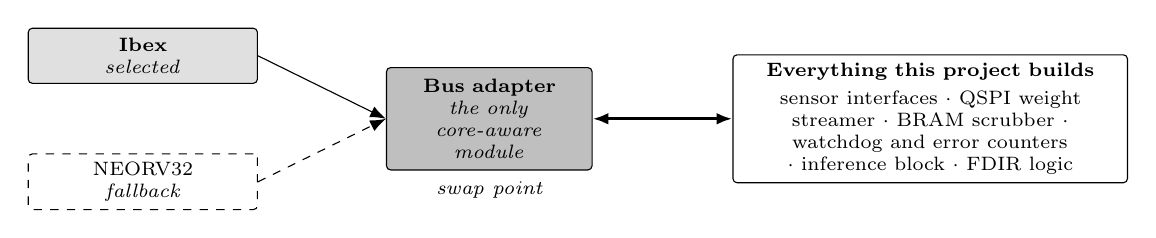
\begin{tikzpicture}[font=\scriptsize]
\node[hard, text width=27mm] (ibex) at (0,1.5) {\textbf{Ibex}\\\itshape selected};
\node[blk, fill=white, text width=27mm, dashed] (neo) at (0,-0.1)
     {NEORV32\\\itshape fallback};
\node[danger, text width=24mm, minimum height=13mm] (ad) at (4.4,0.7)
     {\textbf{Bus adapter}\\\itshape the only core-aware\\\itshape module};
\node[soft, text width=48mm, minimum height=13mm] (mods) at (10.0,0.7)
     {\textbf{Everything this project builds}\\[2pt]
      sensor interfaces \(\cdot\) QSPI weight streamer \(\cdot\)
      BRAM scrubber \(\cdot\) watchdog and error counters \(\cdot\)
      inference block \(\cdot\) FDIR logic};
\draw[ar] (ibex.east) -- (ad.west);
\draw[ar, dashed] (neo.east) -- (ad.west);
\draw[arr, very thick] (ad) -- (mods);
\node[lbl, below=1mm of ad] {swap point};
\end{tikzpicture}
\caption{The bus adapter confines core-specific logic to one module. Switching
base cores means rewriting the adapter, not the system: an estimated few days
rather than the months a full re-integration would cost. This is what makes the
NEORV32 fallback in Table~\ref{tab:cores} a genuine option rather than a
formality.}
\label{fig:adapter}
\end{figure}

Two consequences follow. The fallback becomes real: if Ibex bring-up stalls, the
switch costs days, and the only loss is configuration~C3 of
Figure~\ref{fig:ladder}, since lockstep would then have to be built rather than
enabled. And the port itself becomes a small result --- running the identical
workload and fault campaign on two different cores through one adapter is a
cleaner comparison than the literature usually manages, because everything except
the core is held constant.

I want to be clear that this is the \emph{only} hedge being taken. A hybrid
design carrying both cores was considered and rejected: their bus interfaces and
memory maps differ enough that it would mean building the integration twice for
no experimental gain.

\paragraph{Deliverable of WP1.}
Ibex running on the Boolean Board with \texttt{SecureIbex} \emph{disabled},
inside an SoC of my own construction, booting a real-time operating system and
executing the motion, thermal and extrusion control loops against a simulated
plant. No protection yet --- that is WP2. This build is configuration~C0 of
Figure~\ref{fig:ladder}, the reference against which every later measurement is
taken, so it is a deliverable in its own right rather than an intermediate step.

\subsection{WP2 --- Make the SoC radiation-tolerant (months 4--7)}
\label{sec:wp2}

WP2 adds protection to the WP1 baseline and measures what each addition costs.
Every mechanism below can be switched on or off when the design is built, which
is what allows a fair comparison: the same processor, the same workload, one
variable at a time.

\paragraph{Protection mechanisms.}
The work divides cleanly into configuration and construction.

\emph{Enabled in Ibex and characterised:} dual-core lockstep with temporal
diversity; register-file ECC with write-enable glitch detection and one-hot
address decoding; instruction-cache ECC; hardened program counter; shadow CSRs
on critical control state. Each is a build-time parameter, which is precisely
what makes the controlled comparison possible.

\emph{Built by this project:} periodic scrubbing of idle block RAM; TMR with
voting on peripheral control finite state machines, which sit outside Ibex's
protection domain; staged watchdog escalation from task through application and
core to system reset; error counters that convert Ibex's alert lines into a
telemetry time series the FDIR layer can reason over
\cite{electronics2023faultawareness}; bus parity, timeout and memory protection;
and redundancy on the inference path, which no existing mechanism covers.

\begin{figure}[htbp]
\centering
\resizebox{\textwidth}{!}{%
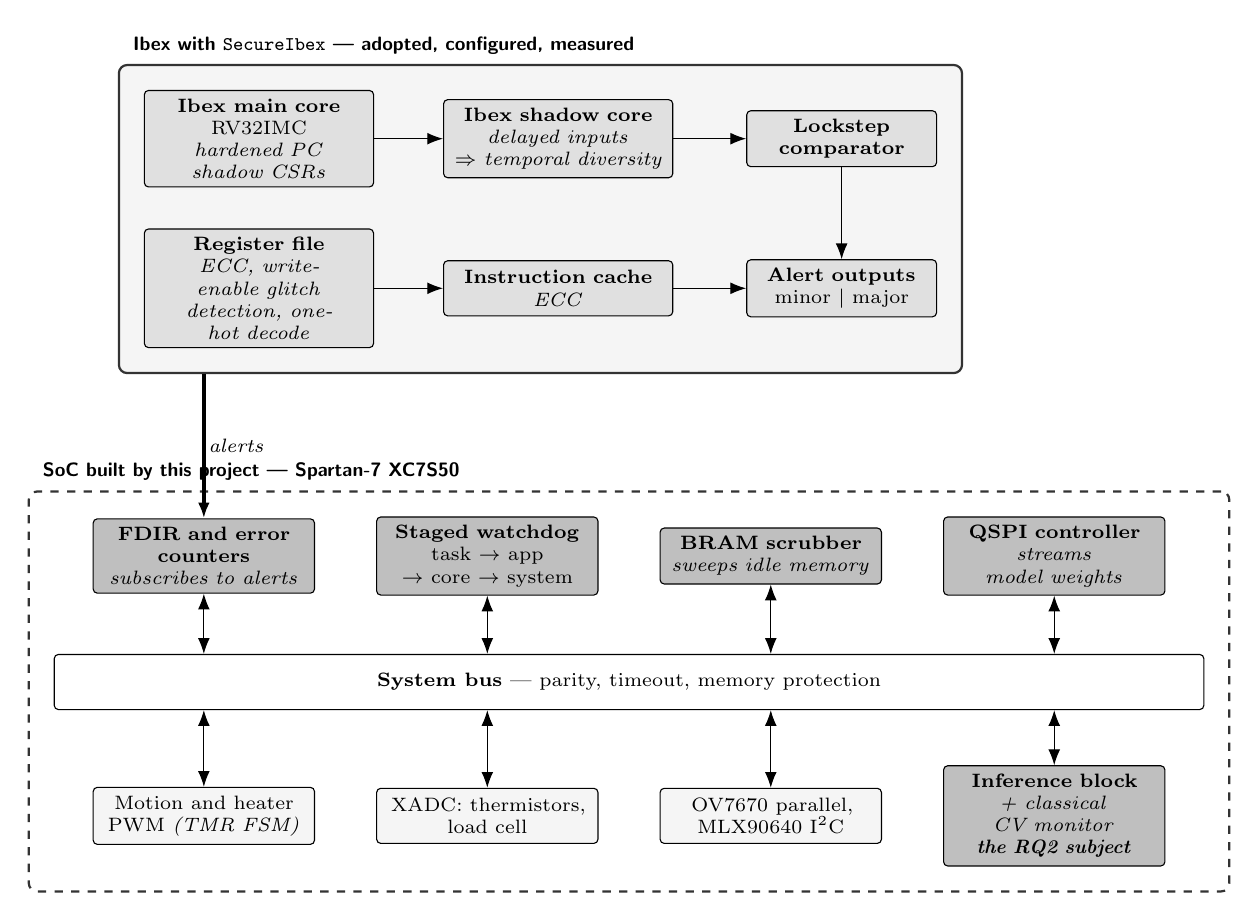
\begin{tikzpicture}[font=\scriptsize]

% ===== IBEX BLOCK =====
\node[hard, text width=27mm] (main) at (2.6,3.4)
     {\textbf{Ibex main core}\\RV32IMC\\\itshape hardened PC\\\itshape shadow CSRs};
\node[hard, text width=27mm] (shadow) at (6.4,3.4)
     {\textbf{Ibex shadow core}\\\itshape delayed inputs\\
      \(\Rightarrow\) temporal diversity};
\node[hard, text width=22mm] (cmp) at (10.0,3.4)
     {\textbf{Lockstep}\\\textbf{comparator}};
\node[hard, text width=27mm] (rf) at (2.6,1.5)
     {\textbf{Register file}\\\itshape ECC, write-enable glitch\\
      \itshape detection, one-hot decode};
\node[hard, text width=27mm] (ic) at (6.4,1.5)
     {\textbf{Instruction cache}\\\itshape ECC};
\node[hard, text width=22mm] (alert) at (10.0,1.5)
     {\textbf{Alert outputs}\\minor \(\mid\) major};

\begin{scope}[on background layer]
  \node[fit=(main)(shadow)(cmp)(rf)(ic)(alert), draw=black!80, thick,
        rounded corners=3pt, inner sep=9pt, fill=black!4] (ibexbox) {};
\end{scope}
\node[anchor=south west, font=\scriptsize\bfseries] at (ibexbox.north west)
     {\hspace{2pt}\textsf{Ibex with \texttt{SecureIbex} --- adopted, configured, measured}};

% ===== PROJECT-BUILT SoC =====
\node[danger, text width=26mm] (fdir) at (1.9,-1.9)
     {\textbf{FDIR and error}\\\textbf{counters}\\
      \itshape subscribes to alerts};
\node[danger, text width=26mm] (wd) at (5.5,-1.9)
     {\textbf{Staged watchdog}\\task \(\rightarrow\) app\\
      \(\rightarrow\) core \(\rightarrow\) system};
\node[danger, text width=26mm] (scrub) at (9.1,-1.9)
     {\textbf{BRAM scrubber}\\\itshape sweeps idle memory};
\node[danger, text width=26mm] (qspi) at (12.7,-1.9)
     {\textbf{QSPI controller}\\\itshape streams model weights};

\node[soft, minimum width=14.6cm] (bus) at (7.3,-3.5)
     {\textbf{System bus} --- parity, timeout, memory protection};

\node[sens, text width=26mm] (mot) at (1.9,-5.2)
     {Motion and heater\\PWM \emph{(TMR FSM)}};
\node[sens, text width=26mm] (adc) at (5.5,-5.2)
     {XADC: thermistors,\\load cell};
\node[sens, text width=26mm] (cam) at (9.1,-5.2)
     {OV7670 parallel,\\MLX90640 I\(^2\)C};
\node[danger, text width=26mm] (inf) at (12.7,-5.2)
     {\textbf{Inference block}\\\itshape + classical CV monitor\\
      \itshape \textbf{the RQ2 subject}};

\begin{scope}[on background layer]
  \node[fit=(fdir)(qspi)(bus)(mot)(inf), draw=black!80, thick, dashed,
        rounded corners=3pt, inner sep=9pt] (socbox) {};
\end{scope}
\node[anchor=south west, font=\scriptsize\bfseries] at (socbox.north west)
     {\hspace{2pt}\textsf{SoC built by this project --- Spartan-7 XC7S50}};

% ===== connections =====
\draw[ar] (main) -- (shadow);
\draw[ar] (shadow) -- (cmp);
\draw[ar] (cmp.south) -- (alert.north);
\draw[ar] (rf.east) -- (ic.west);
\draw[ar] (ic.east) -- (alert.west);
\draw[ar, very thick] (ibexbox.south -| fdir.north) -- (fdir.north)
      node[midway, right, lbl] {alerts};
\foreach \n in {fdir,wd,scrub,qspi}{\draw[arr] (\n.south) -- (\n.south |- bus.north);}
\foreach \n in {mot,adc,cam,inf}{\draw[arr] (\n.north) -- (\n.north |- bus.south);}
\end{tikzpicture}}
\caption{System architecture, drawn to separate what is adopted from what is
built. The solid box is Ibex with \texttt{SecureIbex} enabled: lockstep with
temporal diversity, register-file and cache ECC, hardened PC and shadow CSRs,
all existing and all exposed through two alert lines. The dashed box is the SoC
this project builds around it, including every mechanism Ibex does not provide
--- scrubbing, watchdog escalation, error-counter telemetry, TMR on peripheral
control logic, and the inference path whose corruption is the subject of RQ2.
Ibex supplies the signalling layer; the contribution is what subscribes to it.}
\label{fig:soc}
\end{figure}

\paragraph{Verification.}
Four layers of checking, from cheapest to strongest. First, the official RISC-V
test suite, run through RISCOF, to confirm the processor obeys the instruction set
correctly. Second, randomly generated programs from \texttt{riscv-dv}, run
simultaneously on my design and on Spike, a trusted software model of RISC-V, so
that any disagreement between the two is caught automatically. Third,
self-checking testbenches for the peripherals and memory, with written targets for
how much of the design each test must exercise. Fourth, where the tools allow it,
mathematical proof that the small critical blocks --- the voters and the
error-correction encoders --- are correct for every possible input, not just the
ones I thought to test.

\paragraph{Target device.}
Two different FPGAs will be used, for two different reasons.

The \textbf{fault-injection platform} is the \textbf{RealDigital Boolean Board},
carrying an AMD Spartan-7 XC7S50-CSGA324, already held by the Department. Being
SRAM-based, its
configuration memory \emph{can} be corrupted --- normally a drawback, but exactly
what is needed here, because it allows faults to be injected deliberately, and it
is the standard way this kind of testing is done
\cite{wilson2019neutron,noelv_proton}. Two properties make this specific device a
good fit rather than merely an available one. First, AMD's \textbf{Soft Error
Mitigation (SEM) IP core} supports Spartan-7 \cite{semip}: it uses the device's
ICAP and FRAME\_ECC primitives to detect, correct and classify configuration-memory
upsets, and --- critically for this project --- it includes a built-in error
\emph{injection} feature intended precisely to evaluate SEU mitigation without
beam time. The configuration-memory half of WP5 therefore rests on a free,
pre-verified, vendor-supported mechanism rather than a harness I would have to
write and then justify. Second, the part is comfortably larger than the Artix-7
XC7A35T that would otherwise have been bought
(Table~\ref{tab:fpgares}), which matters for the reason given below.

The board's peripheral set happens to suit the work well. Four Pmod ports across
two 30-pin connectors expose 44 FPGA I/O pins, which is enough for the entire
sensor suite over I\(^2\)C and SPI. An on-board XADC reads the thermistors and
load cell without external conversion. The HDMI output can display live layer
imagery and classifier verdicts, which makes the system demonstrable at review
gates without a host PC. The sixteen slide switches and LEDs are a convenient
front panel for selecting hardening configurations and triggering fault
injection by hand during bring-up.

\paragraph{One real constraint: no external DRAM.}
The Boolean Board carries \SI{128}{\mega\bit} of QSPI flash but \emph{no} DDR3,
unlike the otherwise similar Urbana and Arty~S7 boards. Everything the processor
executes must therefore live in on-chip block RAM ---
\SI{2.7}{\mega\bit}, about \SI{337}{\kilo\byte} --- shared between program code,
stack, frame buffers and neural-network weights. This is a genuine limit and it
shapes three decisions:

\begin{itemize}
  \item \textbf{It settles the base-core choice.} An application-class core such
        as CVA6 expects external DRAM and is simply not an option here. NEORV32
        is designed for exactly this situation: a microcontroller-class SoC
        running from on-chip memory. What was a preference in
        Table~\ref{tab:cores} is now close to a requirement, which removes a
        decision from month~2 rather than adding one.
  \item \textbf{Weights stream from QSPI.} \SI{128}{\mega\bit} is
        \SI{16}{\mega\byte} --- ample for a quantised model. Weights are stored
        in flash and streamed layer by layer into block RAM during inference,
        rather than being resident. This is the standard approach for embedded
        inference on memory-constrained parts.
  \item \textbf{It caps the inspection resolution.} At \(320\times240\)
        greyscale a frame is \SI{75}{\kilo\byte}, so double-buffering plus code
        and working weights fits within the \SI{337}{\kilo\byte} budget with
        room to spare. Higher resolution would not. This is an acceptable
        limit --- published FFF defect classifiers operate at comparable
        resolutions \cite{saluja2020warping} --- but it is a limit, and it is
        recorded as risk R12 rather than discovered later.
\end{itemize}

The camera is chosen to match: an OV7670 with an 8-bit parallel interface, which
maps onto a 30-pin Pmod connector directly. A MIPI CSI-2 module such as the
Raspberry Pi camera would need a bridge the Boolean Board does not have.

The \textbf{flight-representative target} remains a flash-based FPGA (Microchip
IGLOO2, SmartFusion2 or PolarFire), which stores its configuration in flash that
radiation cannot flip, so an entire category of failure disappears. That is
exactly why such devices are used in space, and the comparison between the two
platforms is part of the result.

\begin{table}[htbp]
\centering
\caption{Resources of the available device against the alternative it replaces.}
\label{tab:fpgares}
\small
\begin{tabularx}{\textwidth}{@{}L{4.6cm} L{3.0cm} L{3.0cm} X@{}}
\toprule
& \textbf{XC7S50}\newline\emph{(in the lab)} &
\textbf{XC7A35T}\newline\emph{(Basys 3)} & \\
\midrule
Logic cells      & 52{,}160 & 33{,}280 & \(+57\%\) \\
6-input LUTs     & 32{,}600 & 20{,}800 & \(+57\%\) \\
Flip-flops       & 65{,}200 & 41{,}600 & \(+57\%\) \\
Block RAM        & \SI{2.7}{\mega\bit} & \SI{1.8}{\mega\bit} & \(+50\%\) \\
DSP slices       & 120 & 90 & useful for quantised inference \\
External DRAM    & none & none & forces an MCU-class core \\
QSPI flash       & \SI{128}{\mega\bit} & \SI{32}{\mega\bit} & holds streamed model weights \\
\bottomrule
\end{tabularx}
\end{table}

\paragraph{Why the device size matters to the hypothesis.}
H1 predicts that selective hardening beats full triple modular redundancy on a
reliability-per-resource basis. On this device that stops being an abstract claim
and becomes a physical constraint. Taking the published figure of roughly
\(5.6\times\) resource cost for full TMR \cite{wilson2019neutron}, a modest
RISC-V core occupying roughly 5{,}000 LUTs unprotected would need
roughly 28{,}000 LUTs fully triplicated --- against the 32{,}600 available.
Full TMR of the processor alone would therefore consume most of the fabric,
leaving little for the inference block and peripherals, whereas selective
hardening should fit comfortably. The device does not merely permit the
experiment; it makes the trade-off that RQ1 asks about immediately visible, and it
is honest to note this is a constraint I will be working against rather than
around.

\paragraph{The configuration ladder --- what is actually measured.}
Because every mechanism is a build-time parameter, WP2 reduces to building the
same processor several times and measuring the difference.
Figure~\ref{fig:ladder} defines the ladder. Each rung is a synthesised bitstream
run against the identical control workload and the identical pre-registered fault
schedule, so the comparison isolates one variable at a time.

\begin{figure}[htbp]
\centering
\resizebox{0.98\textwidth}{!}{%
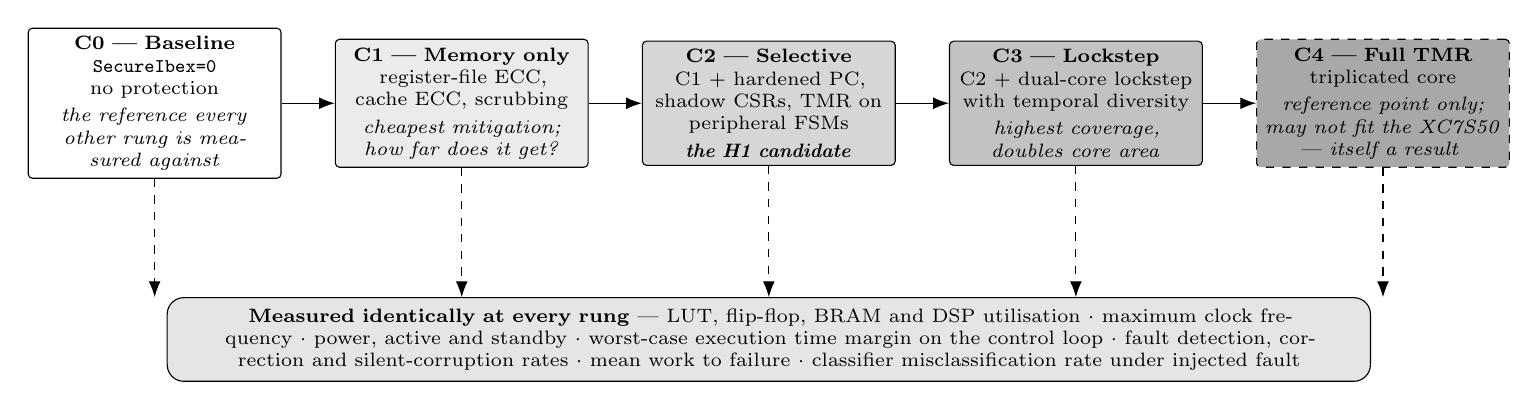
\begin{tikzpicture}[font=\scriptsize]

\node[blk, fill=white, text width=30mm] (c0) at (0,0)
     {\textbf{C0 --- Baseline}\\
      \texttt{SecureIbex=0}\\
      no protection\\[2pt]
      \itshape the reference every\\\itshape other rung is measured against};

\node[blk, fill=black!8, text width=30mm] (c1) at (3.9,0)
     {\textbf{C1 --- Memory only}\\
      register-file ECC,\\
      cache ECC, scrubbing\\[2pt]
      \itshape cheapest mitigation;\\\itshape how far does it get?};

\node[blk, fill=black!16, text width=30mm] (c2) at (7.8,0)
     {\textbf{C2 --- Selective}\\
      C1 \(+\) hardened PC,\\
      shadow CSRs, TMR on\\peripheral FSMs\\[2pt]
      \itshape \textbf{the H1 candidate}};

\node[blk, fill=black!24, text width=30mm] (c3) at (11.7,0)
     {\textbf{C3 --- Lockstep}\\
      C2 \(+\) dual-core lockstep\\
      with temporal diversity\\[2pt]
      \itshape highest coverage,\\\itshape doubles core area};

\node[blk, fill=black!34, text width=30mm, dashed] (c4) at (15.6,0)
     {\textbf{C4 --- Full TMR}\\
      triplicated core\\[2pt]
      \itshape reference point only;\\
      \itshape may not fit the XC7S50\\
      \itshape --- itself a result};

\foreach \a/\b in {c0/c1, c1/c2, c2/c3, c3/c4}{\draw[ar] (\a) -- (\b);}

\node[term, text width=150mm] (meas) at (7.8,-3.0)
     {\textbf{Measured identically at every rung} --- LUT, flip-flop, BRAM and DSP
      utilisation \(\cdot\) maximum clock frequency \(\cdot\) power, active and standby \(\cdot\)
      worst-case execution time margin on the control loop \(\cdot\) fault
      detection, correction and silent-corruption rates \(\cdot\) mean work to
      failure \(\cdot\) classifier misclassification rate under injected fault};

\foreach \n in {c0,c1,c2,c3,c4}{\draw[ar, dashed] (\n.south) -- (\n.south |- meas.north);}
\end{tikzpicture}}
\caption{The configuration ladder. Ibex's parameters make the independent
variable genuinely independent: the same RTL, the same workload and the same
fault schedule, with one protection mechanism added per rung. H1 predicts that
C2 approaches C3's mean work to failure at substantially lower cost, and that C4
either fails to fit or violates the control loop's real-time deadlines --- in
which case that is a finding rather than a failure.}
\label{fig:ladder}
\end{figure}

\paragraph{Deliverable of WP2.}
Five synthesised configurations and the table comparing them: resource cost,
speed penalty, power, real-time margin, and how many injected faults each
catches. This answers the first half of RQ1 on its own, before the printer
exists --- which is why WP1 and WP2 together constitute the descope floor of
Section~11.

\subsection{WP3 --- Design and build the printer (months 3--7)}

This runs alongside WP1 and WP2 because it involves ordering parts and waiting
for them, and that waiting should overlap with design work rather than follow it.

\paragraph{Design.} The machine is modelled completely in SolidWorks first: a
CoreXY motion frame in aluminium extrusion, an \emph{evacuable} build chamber
with O-ring sealing and electrical and fluid feedthroughs, a liquid-cooled hot
end, a temperature-controlled build plate, resistive film wall heaters, a
tension-controlled filament path, and mounts for every sensor. Working in CAD
before cutting metal matters more than usual here, for two reasons: sensor
positions --- particularly the camera angles and the thermal array's field of
view --- have to be right for the imaging to be repeatable and are painful to
change afterwards; and every penetration through a vacuum boundary has to be
planned rather than added later.

\paragraph{Analysis.} The CAD model feeds ANSYS. Structural analysis checks frame
stiffness, finds resonances that would blur the layer imagery or shake the
extruder, and sizes the chamber wall against one atmosphere of external pressure.
Thermal analysis is run in the three configurations of Section~\ref{sec:tools} to
set build-plate power, wall temperature and dwell time. This is the step that
makes the machine microgravity-representative by design rather than by
assertion.

\paragraph{Trade study: conducting heat off a moving hot end.} This is the one
genuinely open mechanical decision in the build, and it is resolved in month~4,
before fabrication, using ANSYS conductance modelling and measured drag on a
single-axis rig. Table~\ref{tab:strap} sets out the options.

\begin{table}[htbp]
\centering
\caption{Options for removing heat from the moving hot end, to be decided in
month~4.}
\label{tab:strap}
\small
\begin{tabularx}{\textwidth}{@{}L{3.0cm} L{3.3cm} L{3.3cm} X@{}}
\toprule
\textbf{Option} & \textbf{Thermal conductance} & \textbf{Cost to the motion
system} & \textbf{Failure and contamination risk} \\
\midrule
Braided copper strap &
Moderate; scales with cross-section, so more heat means more stiffness &
Adds a position-dependent restoring force; the stiffer the strap, the worse the
following error &
Very low. No fluid, no wick, no moving parts. Fatigue over many cycles is the
only concern \\
Heat pipe with a\newline compliant section &
High effective conductance for its mass &
Low if the pipe is mounted along the carriage; bend radius is the constraint &
Wick performance degrades if the pipe is flexed repeatedly; heat pipes are
designed to be rigid \\
Fluid loop with a\newline service loop &
Highest; this is what the published vacuum-FFF systems use
\cite{scirep2025vacuumfff} &
Tubing drag plus the mass of the coolant &
Highest. A leak inside an evacuated chamber is a contamination event, and the
pump is a wear item \\
\bottomrule
\end{tabularx}
\end{table}

\medskip\noindent
The expected outcome is a braid as the baseline, with a heat pipe carrying heat
along the carriage to the braid attachment point if the conductance proves
insufficient. The fluid loop is retained only as a fallback, because a leak into
the chamber is the worst failure mode available and a pump reintroduces exactly
the wear item the design is trying to remove. The measured following error under
each option is reported either way --- it is a small result that anyone building
a vacuum-capable FFF machine would want.

\paragraph{Build.} Fabrication, wiring, and bring-up of the motion and thermal
hardware under a conventional controller at atmospheric pressure first, so that
the mechanics are known to work before either the vacuum or the SoC is
introduced. Pump-down and leak checking follow, then the pressure sweep of
Section~3.5. Only then are the sensors added:

\begin{itemize}
  \item cameras looking down at each layer and across it at an angle, under
        lighting I control so images are comparable from print to print;
  \item an infrared array and thermistors, to see how the part is cooling;
  \item an accelerometer and a contact microphone, since a clogged nozzle, a jam
        or a worn belt each make a distinctive sound and vibration;
  \item an encoder and load cell on the filament, to catch slipping feed and
        measure how hard the extruder is pushing;
  \item chamber pressure and fume sensors, to confirm the enclosure is sealed.
\end{itemize}

ABS will be used for day-to-day development because it is cheap. A small quantity
of polycarbonate will be bought for comparison, since it is closer to the
materials actually printed on the ISS \cite{issnl_amf}.

\paragraph{Deliverable of WP3.} A working, fully instrumented printer producing
repeatable parts under a conventional controller, with CAD, analysis results and
fabrication drawings documented. Note that this deliverable stands alone: it is
useful to the Department as a research testbed regardless of what happens to the
rest of the project.

\subsection{WP4 --- Integrate and test (months 7--9)}

WP4 is where the two threads meet: the protected processor from WP2 takes over
the printer from WP3. The control laws are designed and validated in MATLAB and
Simulink first --- plant models identified from measured step responses of the
real machine, controllers tuned and discretised, stability margins checked, and
the whole loop run in hardware-in-the-loop before the SoC is given authority over
the heaters. The Simulink plant model is then kept as the reference that sensor
residuals are measured against, which is what makes the process-fault branch of
Figure~\ref{fig:fdir} work.

\begin{itemize}
  \item \textbf{The fast loop, on the processor:} deterministic motion, thermal
        and extrusion control, with worst-case execution time analysis
        establishing real-time margins.
  \item \textbf{The slow loop, once per layer:} optical and thermal inspection
        \(\rightarrow\) defect classification \(\rightarrow\) corrective action
        (flow-rate adjustment, temperature adjustment, layer reprint, retract and
        purge, abort).
  \item \textbf{Classifier:} a transfer-learned convolutional network, quantised
        for the SoC, targeting stringing, over- and under-extrusion, warping and
        layer shift --- replicating published systems reporting roughly
        \SIrange{90}{93}{\percent} accuracy
        \cite{saluja2020warping,cirp2024closedloop}, with the critical addition
        that this one runs on hardened hardware under injected fault.
  \item \textbf{Redundant classical computer-vision monitor} as an independent
        check on the learned path --- itself an RQ2 mitigation to be evaluated
        rather than merely an engineering convenience.
  \item \textbf{Hardware safety envelope:} any corrective action capable of
        producing a hazard (over-temperature, unbounded retry, loss of
        containment) is inhibited independently of software.
\end{itemize}

\begin{figure}[htbp]
\centering
\resizebox{0.97\textwidth}{!}{%
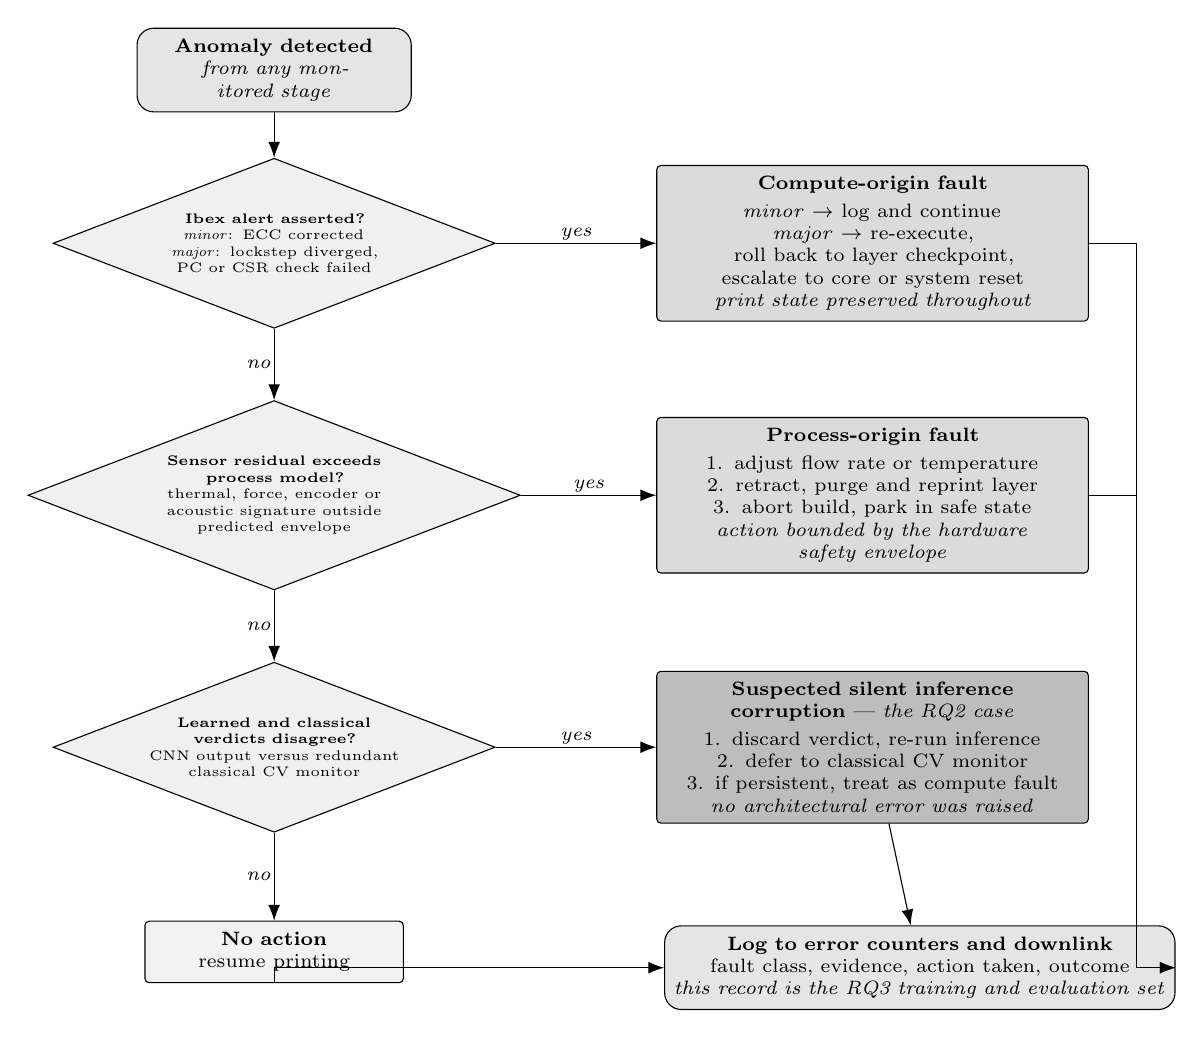
\begin{tikzpicture}[font=\scriptsize]

\node[term, text width=32mm] (start) at (0,0)
     {\textbf{Anomaly detected}\\\itshape from any monitored stage};

\node[dec, text width=34mm] (d1) at (0,-2.2)
     {\textbf{Ibex alert asserted?}\\
      \emph{minor}: ECC corrected\\
      \emph{major}: lockstep diverged,\\
      PC or CSR check failed};

\node[dec, text width=34mm] (d2) at (0,-5.4)
     {\textbf{Sensor residual exceeds\\process model?}\\
      thermal, force, encoder or\\acoustic signature outside\\predicted envelope};

\node[dec, text width=34mm] (d3) at (0,-8.6)
     {\textbf{Learned and classical\\verdicts disagree?}\\
      CNN output versus redundant\\classical CV monitor};

\node[rec, fill=black!5, text width=30mm] (cont) at (0,-11.2)
     {\textbf{No action}\\resume printing};

\node[rec, fill=black!14, text width=52mm] (r1) at (7.6,-2.2)
     {\textbf{Compute-origin fault}\\[2pt]
      \emph{minor} \(\rightarrow\) log and continue\\
      \emph{major} \(\rightarrow\) re-execute,\\
      roll back to layer checkpoint,\\
      escalate to core or system reset\\
      \itshape print state preserved throughout};

\node[rec, fill=black!14, text width=52mm] (r2) at (7.6,-5.4)
     {\textbf{Process-origin fault}\\[2pt]
      1. adjust flow rate or temperature\\
      2. retract, purge and reprint layer\\
      3. abort build, park in safe state\\
      \itshape action bounded by the hardware\\
      \itshape safety envelope};

\node[rec, fill=black!26, text width=52mm] (r3) at (7.6,-8.6)
     {\textbf{Suspected silent inference}\\\textbf{corruption} --- \emph{the RQ2 case}\\[2pt]
      1. discard verdict, re-run inference\\
      2. defer to classical CV monitor\\
      3. if persistent, treat as compute fault\\
      \itshape no architectural error was raised};

\node[term, text width=62mm] (log) at (8.2,-11.4)
     {\textbf{Log to error counters and downlink}\\
      fault class, evidence, action taken, outcome\\
      \itshape this record is the RQ3 training and evaluation set};

\draw[ar] (start) -- (d1);
\draw[ar] (d1) -- node[lbl, left] {no} (d2);
\draw[ar] (d2) -- node[lbl, left] {no} (d3);
\draw[ar] (d3) -- node[lbl, left] {no} (cont);
\draw[ar] (d1) -- node[lbl, above] {yes} (r1);
\draw[ar] (d2) -- node[lbl, above] {yes} (r2);
\draw[ar] (d3) -- node[lbl, above] {yes} (r3);
\draw[ar] (r1.east) -- ++(0.6,0) |- (log.east);
\draw[ar] (r2.east) -- ++(0.6,0) |- (log.east);
\draw[ar] (r3) -- (log);
\draw[ar] (cont) |- (log.west);
\end{tikzpicture}}
\caption{Fault detection, discrimination and recovery. The ordering of the tests
is deliberate: an Ibex alert is unambiguous and is therefore checked first, and
its minor/major distinction already separates corrected from uncorrectable
faults. Process faults, by contrast, must be inferred from sensor residuals
against a model. The third test exists only because of Gap~2 --- an upset in the
inference path raises no error signal and produces no residual anomaly, so the
only remaining evidence is disagreement between the learned and classical
verdicts. RQ3 asks how reliably the second and third branches can be separated
from the first.}
\label{fig:fdir}
\end{figure}

\paragraph{Deliverable of WP4.}
An integrated machine that prints unattended, detects at least four classes of
defect and corrects them without intervention, all under the protected processor.

\subsection{WP5 --- System-level testing (months 9--12)}

This constitutes the scientific core of the project.

\paragraph{Compute-fault injection, at two levels within scope.}
\begin{enumerate}
  \item RTL simulation: single- and multiple-bit upsets injected into flip-flops
        and memory arrays, statistically sampled with reported confidence
        intervals.
  \item FPGA emulation: configuration-memory bit-flipping on the Spartan-7 using
        the AMD SEM IP core, whose error-injection feature exists precisely to
        evaluate SEU mitigation without beam time \cite{semip}; user-memory and
        register injection via a shadow-injection harness.
\end{enumerate}

\paragraph{Beam testing (outside the twelve months; the natural continuation).}
IUAC New Delhi operates the national heavy-ion facility used by ISRO for
single-event-effects qualification of microelectronics \cite{iuac_annual2024},
and allocates beam time to university researchers through a formal proposal
process. Approaching IUAC with a completed, characterised design and published
emulation results is a far stronger proposition than approaching them with an
intention. \textbf{The project does not depend upon beam access, and no
radiation-hardness claim will be advanced on the basis of emulation alone};
results are reported as fault-injection cross-section proxies with the limitation
stated explicitly.

\paragraph{Process-fault injection.}
Reproducible physical faults: filament runout, induced partial nozzle clog,
commanded layer shift, adhesion loss, feed slip and thermal excursion.

\begin{figure}[htbp]
\centering
\resizebox{\textwidth}{!}{%
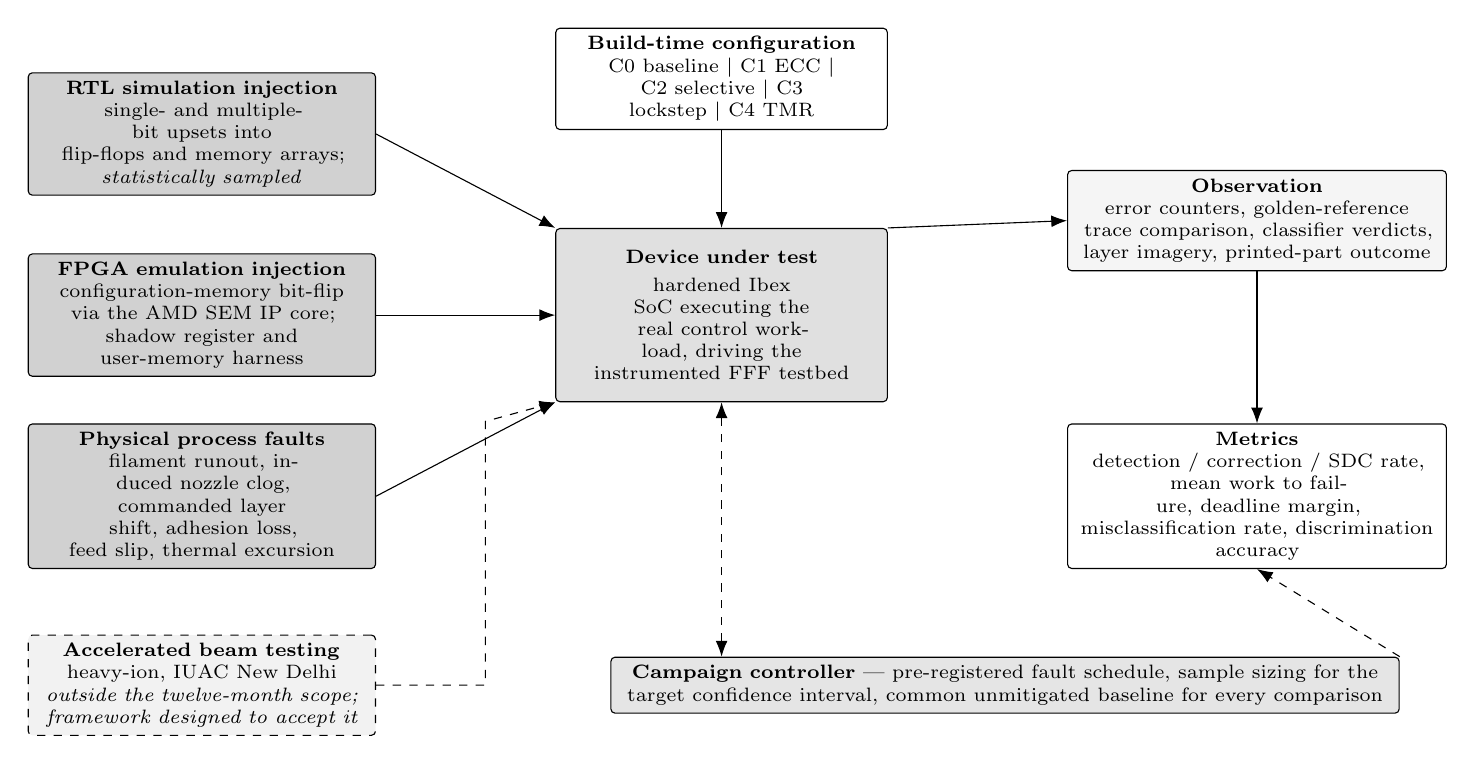
\begin{tikzpicture}[font=\scriptsize]

\node[blk, fill=black!18, text width=42mm] (i1) at (0,2.3)
     {\textbf{RTL simulation injection}\\
      single- and multiple-bit upsets into\\
      flip-flops and memory arrays;\\
      \itshape statistically sampled};

\node[blk, fill=black!18, text width=42mm] (i2) at (0,0)
     {\textbf{FPGA emulation injection}\\
      configuration-memory bit-flip\\
      via the AMD SEM IP core;\\
      shadow register and\\
      user-memory harness};

\node[blk, fill=black!18, text width=42mm] (i3) at (0,-2.3)
     {\textbf{Physical process faults}\\
      filament runout, induced nozzle clog,\\
      commanded layer shift, adhesion loss,\\
      feed slip, thermal excursion};

\node[blk, fill=black!5, text width=42mm, dashed] (i4) at (0,-4.7)
     {\textbf{Accelerated beam testing}\\
      heavy-ion, IUAC New Delhi\\
      \itshape outside the twelve-month scope;\\
      \itshape framework designed to accept it};

\node[soft, text width=40mm] (cfg) at (6.6,3.0)
     {\textbf{Build-time configuration}\\
      C0 baseline \(\mid\) C1 ECC \(\mid\)\\
      C2 selective \(\mid\) C3 lockstep \(\mid\) C4 TMR};

\node[hard, text width=40mm, minimum height=22mm] (dut) at (6.6,0)
     {\textbf{Device under test}\\[2pt]
      hardened Ibex SoC executing the\\
      real control workload, driving the\\
      instrumented FFF testbed};

\node[sens, text width=46mm] (obs) at (13.4,1.2)
     {\textbf{Observation}\\
      error counters, golden-reference\\
      trace comparison, classifier verdicts,\\
      layer imagery, printed-part outcome};

\node[soft, text width=46mm] (met) at (13.4,-2.3)
     {\textbf{Metrics}\\
      detection / correction / SDC rate,\\
      mean work to failure, deadline margin,\\
      misclassification rate, discrimination\\accuracy};

\node[blk, fill=black!10, text width=98mm] (ctrl) at (10.2,-4.7)
     {\textbf{Campaign controller} --- pre-registered fault schedule, sample sizing for
      the target confidence interval, common unmitigated baseline for every comparison};

\draw[ar] (i1.east) -- (dut.north west);
\draw[ar] (i2) -- (dut);
\draw[ar] (i3.east) -- (dut.south west);
\draw[ar, dashed] (i4.east) -- (3.6,-4.7) -- (3.6,-1.35) -- (dut.south west);
\draw[ar] (cfg) -- (dut);
\draw[ar] (dut.north east) -- (obs.west);
\draw[ar] (obs) -- (met);
\draw[arr, dashed] (ctrl.north -| dut.south) -- (dut.south);
\draw[ar, dashed] (ctrl.north east) -- (met.south);
\end{tikzpicture}}
\caption{Fault-injection framework. Three injection routes drive a single device
under test whose mitigations are selected at build time, so that every
configuration is compared against a common unmitigated baseline under an
identical, pre-registered fault schedule. The framework is deliberately
structured so that accelerated beam testing can be added later as a fourth
injection route without altering the measurement or analysis path.}
\label{fig:injection}
\end{figure}

\paragraph{Experimental rigour.}
Every configuration comparison is executed against a common baseline build with
all mitigations disabled. Sample sizes are determined in advance for the target
confidence interval, and the fault-injection schedule is fixed before the
campaign commences. Ground control specimens are printed from a common feedstock
lot under identical documented settings --- the methodological discipline that
rendered the NASA Phase~I and Phase~II results interpretable
\cite{prater2019zerog}.

%=======================================================================
\section{Power}
\label{sec:power}
%=======================================================================

Power is treated separately from thermal design because the two domains involved
differ by two orders of magnitude and are limited by different things. Confusing
them is how in-space manufacturing concepts end up proposing printers that no
spacecraft could run.

\subsection{Two domains, deliberately kept apart}

\begin{table}[htbp]
\centering
\caption{The two power domains. They are not comparable, and the design
consequences run in opposite directions.}
\label{tab:powerdomains}
\small
\begin{tabularx}{\textwidth}{@{}L{3.0cm} L{3.4cm} X@{}}
\toprule
& \textbf{Domain A: the controller} & \textbf{Domain B: the manufacturing unit} \\
\midrule
What it is & Hardened RISC-V SoC on FPGA & Heaters, motion, feedstock handling \\
Bench figure & \SIrange{2}{5}{\watt} & \SIrange{200}{250}{\watt} steady;
\(\approx\)\SI{1}{\kilo\watt} peak during warm-up \\
Dominated by & Logic switching and memory & Resistive heating, overwhelmingly \\
Limited by & \emph{Fabric}, not power & \emph{Power}, absolutely \\
Hardening effect & Multiplies this domain & Unaffected \\
\bottomrule
\end{tabularx}
\end{table}

\paragraph{The consequence, which is not obvious until the numbers are done.}
The manufacturing unit draws roughly fifty to a hundred times the controller.
Tripling the processor's power through full triple modular redundancy therefore
moves the \emph{system} power budget by well under one percent. \textbf{Power is
not a reason to hold back on hardening the processor; fabric is.} This makes the
RQ1 trade-off asymmetric in a way the literature does not discuss, and it is
worth stating plainly because it cuts partly against H1: the resource argument
for selective hardening survives, since the XC7S50 has 32{,}600 LUTs and full
TMR would consume most of them, but the power argument for it does not. Both are
measured; they are expected to disagree; and the disagreement is a result.

\subsection{Domain A: powering and measuring the controller}

\paragraph{Measurement.} Power is added to the metrics recorded at every rung of
the configuration ladder (Figure~\ref{fig:ladder}), by two independent means:
Vivado's vector-based \texttt{report\_power} driven by simulation activity from
the real control workload, and an inline USB power meter on the Boolean Board's
supply. The absolute figures from an FPGA are not the figures a flight ASIC would
show --- FPGA fabric is far less efficient than dedicated silicon --- so
\emph{only the differential across configurations is claimed}. Everything except
the bitstream is held constant, which makes the comparison valid even though the
absolute number is not transferable.

\paragraph{A prediction worth recording in advance.} The power penalty of
hardening should be \emph{sublinear} in the area penalty, because the Ibex core
is a small fraction of total system power once memory, I/O and the inference
block are counted. Lockstep doubles the core but should move system power far
less than double. If this holds, it is a useful result for anyone sizing a
hardened controller, and it is not something the existing literature reports,
which quantifies hardening in LUTs and megahertz rather than watts.

\paragraph{Powering the chip in flight.} A spacecraft supplies an unregulated
battery bus, typically \SIrange{12}{28}{\volt}, from which point-of-load
converters derive the core, I/O and memory rails. Two points matter and both are
noted as scope boundaries rather than work items. First, the regulators must
themselves be radiation-tolerant: hardening the processor achieves nothing if a
single-event latch-up in a point-of-load converter destroys the board. Second,
latch-up protection --- current limiting with autonomous power cycling --- is a
board-level function, not an RTL one, and sits outside this project. Both are
recorded here so that the boundary of what is being claimed is explicit.

\subsection{Domain B: powering the manufacturing unit}

\begin{table}[htbp]
\centering
\caption{Power budget, separating the ground testbed from what a flight unit
would draw. The distinction matters: the pump exists only to manufacture, on the
ground, an environment that orbit supplies free.}
\label{tab:powerbudget}
\small
\begin{tabularx}{\textwidth}{@{}L{3.9cm} L{1.7cm} L{1.9cm} L{1.7cm} X@{}}
\toprule
\textbf{Load} & \textbf{Ground,}\newline\textbf{in air} &
\textbf{Ground, at}\newline\SI{1}{\milli\bar} & \textbf{Flight} &
\textbf{Note} \\
\midrule
Heated bed & \SI{100}{\watt} & \SI{40}{\watt} & \SI{40}{\watt} &
Hold power; \(\approx\)\SI{360}{\watt} during warm-up \\
Chamber heater & \SI{80}{\watt} & \SI{25}{\watt} & \SI{25}{\watt} &
No convective loss below \(\approx\)\SI{10}{\milli\bar} \\
Hotend & \SI{40}{\watt} & \SI{40}{\watt} & \SI{40}{\watt} & Unchanged \\
Steppers (outside chamber) & \SI{32}{\watt} & \SI{32}{\watt} & \SI{32}{\watt} &
Externally mounted; see below \\
Controller and sensors & \SI{10}{\watt} & \SI{10}{\watt} & \SI{10}{\watt} &
Domain A \\
\textbf{Vacuum pump} & --- & \SI{370}{\watt} & \textbf{---} &
\textbf{Ground test equipment only} \\
\midrule
\textbf{Steady} & \(\approx\)\SI{260}{\watt} & \(\approx\)\SI{150}{\watt} &
\(\approx\)\SI{150}{\watt} & Pump off once the chamber is sealed \\
\textbf{Peak (warm-up)} & \(\approx\)\SI{600}{\watt} &
\(\approx\)\SI{970}{\watt} & \(\approx\)\SI{600}{\watt} &
Ground peak includes simultaneous pump-down \\
\bottomrule
\end{tabularx}
\end{table}

\paragraph{These figures are estimates, and are stated as such.}
Every number in Table~\ref{tab:powerbudget} is a component-rating calculation,
not a measurement. Nothing has been built, so the totals carry the usual
uncertainty of a paper exercise: heater duty cycles depend on insulation quality
and chamber leak rate, and the reduction in hold power under vacuum is a
prediction from the thermal argument of Section~\ref{sec:thermal} rather than an
observation. Measuring the real figures is part of WP3, and the difference
between predicted and measured hold power is a small result in its own right.

For a sense of scale, NASA's 3D~Print --- the first printer flown to the ISS, in
2014 --- drew \SI{176}{\watt}, massed \SI{20}{\kilo\gram} and had a
\(6\times12\times6\,\)cm build volume, running ABS \cite{ismoverview2018}. The
estimate here sits in the same band for a machine of broadly similar class,
which is weak evidence that the budget is not wildly wrong. It is no more than
that: 3D~Print operated in cabin air inside the Microgravity Science Glovebox,
so it had convective cooling and convective loss, whereas this design has
neither. The two thermal regimes are different enough that the comparison
establishes an order of magnitude and nothing finer. The later ISS facility,
AMF, is installed in an EXPRESS Rack, and the planned multi-material FabLab is
constrained to \SI{2}{\kilo\watt} peak by rack limits rather than by the
printer's own draw \cite{ismoverview2018}.

\paragraph{The pump is test equipment, not a subsystem.}
This is worth stating plainly because it inverts the usual relationship between
a testbed and the thing it represents. On the ground, roughly \SI{370}{\watt}
and a rotary-vane pump are needed to \emph{create} an environment that an
unpressurised orbital platform provides permanently and for nothing --- and
provides far better, since ambient pressure in low Earth orbit is orders of
magnitude below the \SI{1}{\milli\bar} this chamber targets. \textbf{In the
flight configuration the pump is deleted and replaced by a vent valve.} The
consequences are all favourable:

\begin{itemize}
  \item \textbf{Peak power falls} from \(\approx\)\SI{970}{\watt} to
        \(\approx\)\SI{600}{\watt}, since pump-down never coincides with
        warm-up.
  \item \textbf{Energy per part falls.} Ground operation pays a pump-down cost
        of roughly \SI{0.09}{\kilo\watt\hour} per cycle that flight does not,
        so the ground figures in Table~\ref{tab:orbitpower} are conservative.
  \item \textbf{A wear item disappears.} A rotary-vane pump has bearings, vanes
        and oil --- exactly the class of component this design has been removing
        elsewhere, for a machine meant to run unattended for weeks.
  \item \textbf{A vibration source disappears.} The pump is switched off during
        printing on the ground anyway, precisely because it would inject
        broadband noise into the accelerometer and acoustic channels used for
        clog detection.
\end{itemize}

Even the enclosure changes role. On the ground it is a pressure vessel holding
one atmosphere of differential. In flight, on an unpressurised platform, it
holds no differential at all and exists only for contamination control and part
retention, so it becomes substantially lighter.

\paragraph{The honest consequence: this thermal design assumes an unpressurised
platform.} If the unit were instead flown inside a pressurised module such as
the ISS, cabin air would be present, convection would return, and either the
chamber would have to be actively evacuated --- reintroducing a pump --- or the
thermal architecture of Section~\ref{sec:thermal} would have to be redesigned
around forced convection, as the existing ISS printers are. The design here
follows from the stated target of Section~2.2: an autonomous unit operating
where crew are absent. That is a deliberate commitment rather than an oversight,
and it should be visible to the reader.



\paragraph{Vacuum cuts the running cost.} The same absence of convection that
complicates cooling also removes the dominant heat-loss path, so holding the
chamber at temperature costs roughly a third of what it does in air. Warm-up
energy is unchanged. The consequence is a scheduling one: \textbf{long
continuous prints are far more energy-efficient than many short ones}, because
warm-up is amortised. This reinforces the point already made about layer dwell
time --- thermal and power management collapse into the same scheduling problem
for the planner running on the SoC.

\paragraph{Motors must sit outside the chamber.} Stepper motors and their drivers
are rated on the assumption of convective cooling. At \SI{1}{\milli\bar} they
overheat --- the same physics that motivates the entire thermal argument, now
working against the design. The CoreXY frame is therefore laid out with motors
mounted externally, driving the stage through belts and rotary feedthroughs. This
is a constraint on the SolidWorks work of WP3 and is far cheaper to honour in CAD
than to discover after fabrication.

\paragraph{Thermoelectric wall cooling is dropped.} An earlier version of this
design specified thermoelectric modules for commanded wall temperature. For ABS
and polycarbonate the chamber wants to be \emph{hot} to prevent warping, so the
cooling mode would almost never be used. Resistive heating with passive loss to
ambient achieves the same control at a fraction of the power, with no H-bridge
and no additional failure mode.

\subsection{What this would mean in orbit}

\begin{table}[htbp]
\centering
\caption{Feasibility of a \SI{150}{\watt} manufacturing unit against platform
power, on the estimated figures of Table~\ref{tab:powerbudget}. One part is taken
as \(\approx\)\SI{1}{\kilo\watt\hour}, being a three-hour print plus warm-up. The
conclusions are robust to a factor-of-two error in the estimate; the boundary
between the marginal and comfortable rows is not.}
\label{tab:orbitpower}
\small
\begin{tabularx}{\textwidth}{@{}L{4.0cm} L{2.6cm} L{2.4cm} X@{}}
\toprule
\textbf{Platform} & \textbf{Orbit-average power} & \textbf{Energy per day} &
\textbf{Verdict} \\
\midrule
3U CubeSat, body-mounted cells & \SIrange{5}{10}{\watt} &
\(\approx\)\SI{0.2}{\kilo\watt\hour} &
Infeasible: one part would consume the entire spacecraft's output for four to
eight days \\
6U--12U with deployable arrays & \SIrange{20}{50}{\watt} &
\SIrange{0.5}{1.2}{\kilo\watt\hour} &
Marginal; viable only for very small parts with aggressive duty cycling \\
ISS internal payload & \(\approx\)\SI{500}{\watt} per locker & continuous &
Comfortable --- and precisely why the only operational in-space printer is on the
ISS \\
Commercial free-flyer & \SIrange{1}{5}{\kilo\watt} & continuous &
Comfortable; the Phase~7 architecture \\
\bottomrule
\end{tabularx}
\end{table}

\paragraph{Sizing a self-powered unit.} Supporting \SI{150}{\watt} orbit-average
in low Earth orbit, where roughly \SI{35}{\percent} of each
\(\approx\)\SI{92}{\minute} orbit is spent in eclipse, requires about
\SI{230}{\watt} generated while sunlit. At the solar constant of
\SI{1361}{\watt\per\metre\squared} and \SI{30}{\percent} triple-junction cell
efficiency, that is roughly \SI{0.6}{\metre\squared} of cell area before pointing
losses, degradation and packing --- realistically closer to
\SI{1}{\metre\squared}. Carrying the load through a \SI{35}{\minute} eclipse
needs on the order of \SI{90}{\watt\hour} of usable battery, some
\SIrange{1}{2}{\kilo\gram} of cells at typical depth of discharge. A
manufacturing payload is therefore not a small addition to a spacecraft; it sizes
the spacecraft.

\paragraph{The design consequence, and why it belongs in this proposal.}
Printing must be synchronised to the orbit: build during the sunlit pass, and
either hold the chamber warm through eclipse at a cost in battery, or accept a
thermal cycle that damages layer adhesion. That is a decision the onboard planner
has to make, against a power forecast, a thermal model and a print queue --- and
it is the same planner already responsible for regulating interlayer temperature
through dwell time (Section~\ref{sec:thermal}). \textbf{Power scheduling and
thermal scheduling are one problem, and it lands on the controller this project
is building.} Implementing an orbit-synchronised planner is beyond the twelve
months, but the control architecture is structured so that the outer loop takes a
resource forecast as an input rather than assuming unlimited power, which is what
makes it extensible to that case rather than a dead end.

%=======================================================================
\section{Work Plan and Milestones}
%=======================================================================

The schedule is built around two constraints. First, the critical path runs
WP0 \(\rightarrow\) WP1 \(\rightarrow\) WP2 \(\rightarrow\) WP5: the system-level
campaign cannot begin until a protected processor exists, and WP1 and WP2 alone
are sufficient to answer RQ1 even if everything downstream fails. Second, WP3 ---
building the printer --- is started in month~3 and run alongside the processor
work rather than after it, because it involves ordering parts and waiting for
them. Overlapping the two means a delivery delay costs slack instead of schedule.
The two threads are developed against an interface frozen at the end of month~2:
a written specification of the commands and telemetry passing between the SoC and
the printer, so that neither side blocks the other.

Each work package ends in something concrete and independently useful --- a
verified processor, a measured protection comparison, a working instrumented
printer, an integrated closed-loop machine, a characterisation dataset --- so
that the project degrades gracefully rather than producing nothing if it stops
early.

Review gates fall quarterly (M2, M5, M8, M11). The month~2 gate is different in
kind from the others: it is a genuine termination point, not a progress review,
and is discussed in Section~\ref{sec:prep}.

\begin{figure}[htbp]
\centering
\begin{ganttchart}[
    x unit=0.92cm,
    y unit title=0.6cm,
    y unit chart=0.58cm,
    vgrid, hgrid,
    title height=1,
    bar height=0.5,
    bar/.append style={fill=black!55},
    milestone/.append style={fill=black},
    bar label font=\footnotesize,
    milestone label font=\footnotesize\itshape,
    title label font=\footnotesize
  ]{1}{12}
  \gantttitle{Month}{12} \\
  \gantttitlelist{1,...,12}{1} \\
  \ganttbar{WP0 Planning}{1}{2} \\
  \ganttbar{WP1 Build the SoC}{2}{5} \\
  \ganttbar{WP2 Radiation tolerance}{4}{7} \\
  \ganttbar{WP3 Design and build printer}{3}{7} \\
  \ganttbar{WP4 Integrate and test}{7}{9} \\
  \ganttbar{WP5 System-level testing}{9}{12} \\
  \ganttmilestone{Review gates}{2} \ganttmilestone{}{5}
  \ganttmilestone{}{8} \ganttmilestone{}{11}
\end{ganttchart}
\caption{Twelve-month work package schedule with quarterly review gates. Each
package terminates in a concrete deliverable before the next depends on it.}
\label{fig:gantt}
\end{figure}

\begin{table}[htbp]
\centering
\caption{Milestones and evidence.}
\label{tab:milestones}
\small
\begin{tabularx}{\textwidth}{@{}c X L{4.4cm}@{}}
\toprule
\textbf{Month} & \textbf{Milestone} & \textbf{Evidence} \\
\midrule
M2  & \textbf{Go/no-go gate (WP0).} Ibex running the compliance suite on the
      Boolean Board; bus adapter defined; printer design frozen in CAD;
      SoC--printer interface specified &
      CI report; live demonstration; adapter specification; SolidWorks model \\
M5  & \textbf{WP1 complete.} Verified unprotected SoC running the control
      workload against a simulated plant; ANSYS structural and thermal analysis
      complete & Live demonstration; analysis report \\
M7  & \textbf{WP2 and WP3 complete.} Protected SoC characterised against the
      baseline; printer built, instrumented and printing repeatably under a
      conventional controller & Resource, timing and fault-injection report;
      working machine \\
M8  & Review gate; SoC drives the printer's motion and thermal loops &
      Live demonstration \\
M9  & \textbf{WP4 complete.} Closed-loop defect detection and correction
      operational; fault-injection framework validated & Accuracy figures;
      open-source release \\
M11 & Review gate; system campaign complete, RQ1 and RQ2 answered; first paper
      submitted & Results report; dataset; submission record \\
M12 & \textbf{WP5 complete.} Report submitted; second paper submitted &
      Documents; artefact release \\
\bottomrule
\end{tabularx}
\end{table}

\paragraph{Contingency.}
Should the printer not be under SoC control by month~8, WP5 is descoped to
compute-fault characterisation against a hardware-in-the-loop simulated control
workload. This continues to address RQ1 and RQ2 and remains publishable. The
descope is declared in advance so that the project may fail gracefully rather
than late.

%=======================================================================
\paragraph{Deliverable of WP5.}
The answers to RQ1 and RQ2 with stated confidence intervals, a released dataset
and fault-injection framework, and the submitted papers.

\section{Expected Outcomes and Contributions}
%=======================================================================

\paragraph{Scientific contributions.}
\begin{enumerate}[leftmargin=*]
  \item First characterisation of RISC-V hardening overhead against a hard
        real-time additive manufacturing control workload, in place of synthetic
        benchmarks.
  \item First quantification of single-event-upset propagation through an
        ML-driven manufacturing control decision, with evaluation of redundancy
        strategies for that path.
  \item A methodology for establishing the microgravity representativeness of a
        ground testbed by means of orientation invariance and process-setting
        control.
  \item \emph{(Extension)} A unified compute/process fault taxonomy and
        discrimination method for autonomous manufacturing systems.
\end{enumerate}

\paragraph{Artefacts, all released open-source.}
\begin{enumerate}[leftmargin=*]\setcounter{enumi}{4}
  \item Hardened, configurable RISC-V SoC RTL with independently selectable
        mitigations.
  \item Fault-injection framework spanning RTL simulation, FPGA emulation and
        physical process faults, reusable by any group undertaking comparable
        work.
  \item Labelled defect dataset with paired hardware error-counter telemetry; no
        comparable dataset presently exists.
\end{enumerate}

\begin{table}[htbp]
\centering
\caption{Planned publications and target venues.}
\label{tab:pubs}
\small
\begin{tabularx}{\textwidth}{@{}X L{6.6cm}@{}}
\toprule
\textbf{Output} & \textbf{Target venue} \\
\midrule
Hardening architecture and fault-injection results &
IEEE International Symposium on VLSI Design and Test (VDAT), VLSI Design
Conference, RADECS, or \emph{Microelectronics Reliability} \\
Closed-loop control under fault; dataset release &
IEEE Aerospace Conference, \emph{Journal of Manufacturing Processes}, or
\emph{Additive Manufacturing} \\
Review and gap analysis \emph{(if time permits)} &
\emph{Acta Astronautica} or \emph{IEEE Access} \\
\bottomrule
\end{tabularx}
\end{table}

\begin{figure}[htbp]
\centering
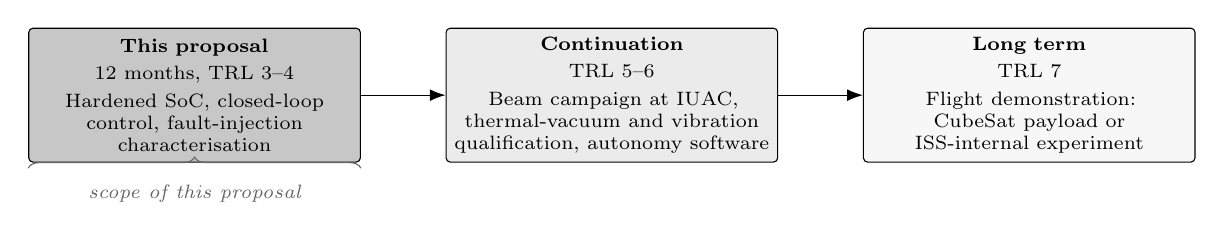
\begin{tikzpicture}[font=\scriptsize]
  \node[blk, fill=black!22, text width=40mm, minimum height=17mm] (p1) at (0,0)
       {\textbf{This proposal}\\[2pt]
        12 months, TRL 3--4\\[2pt]
        Hardened SoC, closed-loop\\control, fault-injection\\characterisation};
  \node[blk, fill=black!8, text width=40mm, minimum height=17mm] (p2) at (5.3,0)
       {\textbf{Continuation}\\[2pt]
        TRL 5--6\\[2pt]
        Beam campaign at IUAC,\\thermal-vacuum and vibration\\qualification, autonomy software};
  \node[blk, fill=black!3, text width=40mm, minimum height=17mm] (p3) at (10.6,0)
       {\textbf{Long term}\\[2pt]
        TRL 7\\[2pt]
        Flight demonstration:\\CubeSat payload or\\ISS-internal experiment};
  \draw[ar] (p1) -- (p2);
  \draw[ar] (p2) -- (p3);
  \draw[decorate, decoration={brace, amplitude=4pt}, black!60]
       ($(p1.south west)+(0,-2pt)$) -- ($(p1.south east)+(0,-2pt)$)
       node[midway, below=5pt, lbl] {scope of this proposal};
\end{tikzpicture}
\caption{Position of the proposed work within a longer trajectory. Only the
first stage is being proposed; it is scoped to stand alone, and produces the
evidence package required to pursue the second.}
\label{fig:roadmap}
\end{figure}

\paragraph{Trajectory.}
This project resides at TRL~3--4 as defined in NPR~7123.1C \cite{npr71231c}. It
constitutes the first phase of a longer roadmap encompassing system architecture,
autonomy software, environmental qualification and eventual flight
demonstration; it is nonetheless deliberately scoped to stand alone. Should the
work proceed no further, it remains a complete and novel contribution. Should it
continue, it constitutes the evidence package for a beam-time proposal to IUAC
and for subsequent funding applications.

%=======================================================================
\section{Resources Requested}
%=======================================================================

\subsection{Equipment and consumables}

The budget is presented as four tranches tied to the review gates, not as a
single request. Each tranche is released only if the previous gate is passed, so
the Department's exposure at any point is bounded by what has already been
demonstrated. If the project is stopped at any gate, the spend to that point has
produced something the Department keeps.

\begin{table}[htbp]
\centering
\caption{Phased budget. Each tranche is contingent on passing the preceding
gate.}
\label{tab:phases}
\small
\begin{tabularx}{\textwidth}{@{}L{1.5cm} L{2.1cm} L{2.0cm} X@{}}
\toprule
\textbf{Tranche} & \textbf{Released} & \textbf{Amt.\ (\rupee)} &
\textbf{What it buys, and what exists if the project stops here} \\
\midrule
\textbf{T1} & At approval & 3{,}000 &
Sensors for characterising the existing printer. Deliverable: instrumented
baseline and a labelled defect dataset. \\
\textbf{T2} & M2 gate passed & 32{,}100 &
Printer build and remaining sensors. Deliverable: a working custom instrumented
printer, retained by the Department as a research testbed. \\
\textbf{T3} & M5 gate passed & 20{,}900 &
Vacuum chamber and thermal control. Deliverable: a convection-free process
chamber and the pressure-sweep result. \\
\textbf{T4} & M7 gate passed & 11{,}500 &
PolarFire Discovery Kit for the flight-representative comparison. Deliverable:
the flash-versus-SRAM measurement. \\
\midrule
\textbf{Total} & & \textbf{67{,}200} & \(\approx\)US\$790 \\
\bottomrule
\end{tabularx}
\end{table}

Two decisions cut this well below what the earlier version of this proposal
assumed. First, the Department already holds a RealDigital Boolean Board
(Spartan-7 XC7S50), so no SRAM-based FPGA is bought; the part is larger than the
Artix-7 board that would otherwise have been specified, and its Pmod ports and
on-board XADC remove the need for a separate sensor-interface board at this
stage (Section~\ref{sec:wp2}). Second, and more significantly, the vacuum requirement
was derived rather than assumed: \SI{1}{\milli\bar} suppresses convection with an
order of magnitude of margin (Section~\ref{sec:thermal}), which is reached by a
single-stage rotary-vane pump at roughly \rupee\,8{,}000 rather than the
\rupee\,22{,}000 two-stage pump needed for \(\SI{e-3}{\milli\bar}\), and needs
only an analogue gauge. Specifying more vacuum than the physics requires would
have cost about a fifth of the budget for no experimental gain.

Where an item is commonly found in university laboratories it is marked
\(^{\ddagger}\), with the borrowed-equipment total given at the foot of
Table~\ref{tab:budget}. Realistically, if a rotary-vane pump can be borrowed from
Physics or Chemistry and a dead printer scavenged for motion hardware, the cash
requirement falls to roughly \rupee\,51{,}700.

\begin{xltabular}{\textwidth}{@{}L{7.4cm} L{1.7cm} X@{}}
\caption{Bill of materials, grouped by tranche. Item names link to the supplier
page. Items marked \(^{\ddagger}\) are commonly available in university
laboratories and may be borrowed rather than bought.}
\label{tab:budget}\\
\toprule
\textbf{Item, part number and supplier} & \textbf{Est.\ (\rupee)} &
\textbf{Purpose} \\
\midrule
\endfirsthead
\multicolumn{3}{@{}l}{\emph{Table \thetable\ continued from previous page}}\\
\toprule
\textbf{Item, part number and supplier} & \textbf{Est.\ (\rupee)} &
\textbf{Purpose} \\
\midrule
\endhead
\midrule
\multicolumn{3}{r@{}}{\emph{continued on next page}}\\
\endfoot
\bottomrule
\endlastfoot

\multicolumn{3}{@{}l}{\textbf{Already held --- no cost}}\\
RealDigital Boolean Board, Spartan-7 XC7S50-CSGA324 \emph{(Department)} & --- &
Fault injection via the SEM IP core; 52{,}160 logic cells; 4 Pmod ports, XADC,
HDMI out \\
Vivado, Libero, Verilator, RISCOF \emph{(free editions)} & --- &
FPGA and verification toolchain \\
SolidWorks, ANSYS, MATLAB \emph{(Institute licences)} & --- &
CAD, analysis and control design \\

\midrule
\multicolumn{3}{@{}l}{\textbf{T1 --- At approval (\rupee\,3{,}000)}}\\
\href{https://robu.in/product/ov7670-camera-module/}{OV7670 camera module}
(8-bit parallel, Pmod-compatible) and LED ring with diffuser
\emph{(Robu.in)} & 1{,}400 &
Layer-wise inspection under controlled lighting; parallel interface avoids the
MIPI bridge the board lacks \\
\href{https://robu.in/product/adxl345-3-axis-digital-gravity-sensor-acceleration-module/}{ADXL345
accelerometer}; piezo contact disc \emph{(Robu.in)} & 900 &
Nozzle clog, jam and wear detection \\
\href{https://robu.in/product/as5600-magnetic-encoder-sensor-module/}{AS5600
magnetic encoder}; NTC thermistors \emph{(Robu.in)} & 700 &
Feed slip; temperature \\

\midrule
\multicolumn{3}{@{}l}{\textbf{T2 --- After the M2 gate (\rupee\,32{,}100)}}\\
Aluminium extrusion, brackets, fasteners \emph{(local)} & 4{,}500 &
CoreXY frame; stiffness set by ANSYS \\
Linear rails, belts, pulleys, idlers\(^{\ddagger}\) \emph{(Robu.in)} & 4{,}000 &
Motion stage \\
4\(\times\) NEMA17 steppers with
\href{https://robu.in/product/tmc2209-stepper-motor-driver-module/}{TMC2209
drivers}\(^{\ddagger}\) \emph{(Robu.in)} & 3{,}500 &
Motion and extrusion axes \\
All-metal hotend (300\(^\circ\)C rated), Bowden extruder \emph{(Robu.in)} &
3{,}500 & High-temperature capability; Bowden keeps the extruder motor outside
the chamber \\
Heated bed; \SI{24}{\volt} \SI{500}{\watt} PSU; MOSFET and solid-state relay
switching; opto-isolators \emph{(Robu.in)} & 4{,}500 &
Bed adhesion and power distribution; isolation between FPGA and power stages \\
Bimetallic thermal cutout, emergency stop, fused mains inlet
\emph{(local)} & 1{,}200 &
Hardware safety chain in series with the heater supply, independent of the
processor (Section~\ref{sec:power}) \\
\href{https://robu.in/product/ina226-i2c-bi-directional-current-power-monitor/}{INA226
current and power monitor} \emph{(Robu.in)} & 400 &
Differential power measurement across ladder configurations \\
\href{https://robu.in/product/waveshare-mlx90640-ir-array-thermal-imaging-camera-32x24-pixels-110-fov/}{Waveshare
MLX90640 IR array}, 32\(\times\)24 px, I\(^2\)C \emph{(Robu.in)} & 4{,}500 &
Layer and bead thermal field \\
1\,kg load cell with
\href{https://robu.in/product/hx711-load-cell-amplifier-module/}{HX711
amplifier}; 2\(\times\) MAX6675 thermocouples \emph{(Robu.in)} & 2{,}000 &
Extrusion force; nozzle temperature \\
\href{https://robu.in/product/bme280-temperature-humidity-barometric-pressure-sensor-module/}{BME280};
MQ-135 VOC sensor \emph{(Robu.in)} & 900 &
Containment and off-gassing \\
ABS filament, 2\,kg \emph{(local)} & 2{,}000 & Development lots \\
Perfboard, connectors, wiring, level shifters \emph{(Robu.in)} & 1{,}100 &
Sensor interface, prototyped before PCB \\

\midrule
\multicolumn{3}{@{}l}{\textbf{T3 --- After the M5 gate (\rupee\,20{,}900)}}\\
Chamber: stainless stock pot or acrylic cylinder, O-ring, acrylic lid,
viewport \emph{(local)} & 4{,}000 &
Build volume; the standard resin-degassing chamber construction \\
Single-stage rotary-vane pump, \SI{1}{\milli\bar}
class\(^{\ddagger}\) \emph{(local / IndiaMART)} & 8{,}000 &
\textbf{Ground test equipment only} --- creates on the bench the vacuum orbit
provides free; deleted in any flight configuration
(Section~\ref{sec:power}) \\
Analogue vacuum gauge and hose \emph{(local)} & 800 &
Pressure as an experimental variable \\
Electrical and fluid feedthroughs \emph{(local)} & 2{,}500 &
Sensor, motor and coolant penetrations \\
Copper heat pipes (sintered wick), braided copper straps
\emph{(Robu.in)} & 1{,}200 &
Heat off the moving hot end; no pump, no moving parts \\
High-emissivity coating; polished foil; aluminised MLI film
\emph{(local)} & 2{,}000 &
Wall emissivity as a design variable; insulation \\
G10 / PEEK standoffs, thermal interface material \emph{(Robu.in)} & 1{,}200 &
Preventing heat leak into the frame \\
Silicone film heaters and PT100 sensors for the chamber wall
\emph{(Robu.in)} & 1{,}400 &
Commanded wall temperature; resistive rather than thermoelectric, since the
chamber is always heated \\
Polycarbonate filament, 1\,kg \emph{(local)} & 3{,}000 &
High-temperature comparison material \\

\midrule
\multicolumn{3}{@{}l}{\textbf{T4 --- After the M7 gate (\rupee\,11{,}500)}}\\
\href{https://www.microchip.com/en-us/development-tool/mpfs-disco-kit}{PolarFire
SoC Discovery Kit}, MPFS-DISCO-KIT (MPFS095T)
\emph{(Microchip Direct)} & 11{,}500 &
Flight-representative target; flash configuration memory is inherently
SEU-immune \\

\midrule
\textbf{Total requested} & \textbf{67{,}200} & \(\approx\)US\$790 \\
\textbf{If \(^{\ddagger}\) items are borrowed} & \textbf{51{,}700} &
\(\approx\)US\$610 \\

\midrule
\multicolumn{3}{@{}l}{\textit{Explicitly deferred}}\\
PEI/ULTEM 9085 filament & --- &
\(\approx\)\rupee\,60{,}000 per kg; sought as a donated sample only when
flight-representative properties must be measured \\
Two-layer sensor PCB \emph{(JLCPCB)} & --- &
\(\approx\)\rupee\,6{,}000; only once the pinout is settled on perfboard \\
Liquid cold-end loop & --- &
\(\approx\)\rupee\,3{,}000; only if conduction proves insufficient
(Table~\ref{tab:strap}) \\
\href{https://www.digikey.in/en/products/detail/digilent-inc/410-324/6133793}{Nexys
A7-100T} \emph{(DigiKey India)} & --- &
\(\approx\)\rupee\,40{,}000; only if the inference block will not fit alongside
a hardened core in the XC7S50 \\
\end{xltabular}

\medskip
Also required: bench instrumentation (oscilloscope, bench supply, logic
analyser) and compute for model training and RTL simulation, both from existing
laboratory stock.

This is deliberately a low-cost proposal, and the phasing is deliberate too. The
novelty resides in the experimental design rather than in expensive equipment,
and no tranche is requested before the preceding gate has demonstrated that it
is warranted.

\subsection{From the supervisor}

\begin{itemize}
  \item \textbf{Technical supervision}, particularly on verification methodology
        and FPGA implementation.
  \item \textbf{Review at the four gates} (M2, M5, M8, M11). I would ask that
        these be adversarial rather than encouraging, and that the M2 gate be
        enforced strictly.
  \item \textbf{Publication guidance} and co-authorship.
  \item \textbf{Institutional introductions} where you judge them appropriate:
        to IUAC New Delhi for eventual beam access, to a materials group for
        micro-computed-tomography and mechanical characterisation of printed
        specimens, or to any student satellite activity. Access relationships
        take longer to establish than hardware.
\end{itemize}

%=======================================================================
\section{Risk Assessment}
%=======================================================================

The risks below are ordered by their expected effect on the twelve-month
deliverable rather than by likelihood alone. Three points are worth stating
explicitly.

First, R1 --- my own inexperience --- is the dominant risk, and it is addressed
structurally rather than by assurance: the planning phase of Section~\ref{sec:prep}, the
month~2 termination gate, and the decisions to adopt rather than author both the
base core and the verification infrastructure. If the risk materialises, it does
so at month~2 at a cost of two months, not at month~10 at a cost of the project.

Second, the mitigations listed are design decisions already embedded in the plan,
not intentions to be acted on if trouble arises. The hardware safety envelope,
the redundant classical computer-vision path and the two-tier objective structure
all exist in the methodology because of the risks they answer.

Third, R6 is included because a negative result is a legitimate outcome here. If
hardening overhead proves incompatible with the control loop's real-time
deadlines, that finding answers RQ1 and is publishable; it is recorded as a risk
only because it would defeat the engineering goal while advancing the research
one.

\begin{table}[htbp]
\centering
\caption{Risk register.}
\label{tab:risks}
\small
\begin{tabularx}{\textwidth}{@{}c L{3.6cm} c c X@{}}
\toprule
\textbf{\#} & \textbf{Risk} & \textbf{Lik.} & \textbf{Imp.} & \textbf{Mitigation} \\
\midrule
R1 & Candidate lacks prior RTL experience & High & High &
Months 1--2 constituted as an explicit preparation phase
(Section~\ref{sec:prep}) with a strict go/no-go gate; Ibex adopted rather than
authored, with its protection mechanisms already implemented and its verification
flow already working; a thin bus adapter (Figure~\ref{fig:adapter}) keeps the
NEORV32 fallback a days-long switch rather than a rebuild \\
R2 & Scope too broad for twelve months & Med & High &
Two-tier objectives (Core/Extension, Table~\ref{tab:objectives}); declared
descope path; each work package ends in a standalone deliverable, so stopping
early still leaves something usable; WP1--WP2 and WP3 run in parallel against an
interface frozen at month~2 \\
R3 & Beam time unobtainable & High & Low &
Beam testing is explicitly outside the twelve-month scope; emulation is the
baseline method, not a fallback; no claim advanced without data \\
R4 & Building the printer consumes disproportionate effort & High & Med &
Standard CoreXY architecture and off-the-shelf motion components --- nothing is
mechanically novel; SolidWorks and ANSYS work completed before ordering; machine
brought up under a conventional controller first, so mechanical and control
problems are separated; hard checkpoint at M7 \\
R5 & Classifier accuracy insufficient after quantisation & Med & Med &
Redundant classical computer-vision path already in the design; a reduced
defect-class scope remains an acceptable outcome and still addresses RQ2 \\
R6 & Hardening overhead violates real-time deadlines & Low & Low &
\emph{This constitutes a finding rather than a failure} --- it directly
addresses RQ1 and is publishable \\
R7 & Flash-based FPGA board procurement delay & Med & Low &
All WP1 and WP2 work proceeds on the Spartan-7 already held by the Department;
the flash device is required only for the flight-representative comparison, which
is the last measurement rather than the first \\
R8 & Fabrication or machining access unavailable & Med & Med &
Design uses extrusion, laser-cut sheet and printed brackets rather than machined
parts; the frame can be assembled with hand tools \\
R9 & Vacuum chamber leaks, or pump unavailable & Med & Med &
Chamber only needs \SI{1}{\milli\bar} class, not high vacuum, so
elastomer seals suffice; the machine functions at atmospheric pressure
throughout, and the pressure sweep is an added measurement rather than a
precondition \\
R10 & Moving thermal link cannot carry the hot-end load without degrading
positioning accuracy & Med & Med &
Resolved by trade study in month~4 before fabrication
(Table~\ref{tab:strap}); the pumped fluid loop used by published vacuum-FFF
systems is retained as a fallback; measured following error reported either way \\
R11 & Polymer outgassing contaminates the chamber or\newline degrades the print &
Med & Low & Reported as manageable in published low-vacuum FFF work
\cite{ceas2021lowvacuum}; cold trap and carbon getter fitted; ABS and PC both
have documented low total mass loss \\
R12 & On-chip memory insufficient for the hardened core plus the inference
block & Med & Med &
\SI{337}{\kilo\byte} of block RAM is the hard limit; weights stream from the
\SI{16}{\mega\byte} QSPI flash rather than residing in BRAM; inspection capped at
\(320\times240\), comparable to published FFF classifiers
\cite{saluja2020warping}; the Nexys A7-100T remains a costed contingency \\
R13 & Bench load approaching \SI{1}{\kilo\watt} during simultaneous warm-up and
pump-down & Med & Low &
Ground-only condition; the pump is test equipment and is off during printing;
warm-up and pump-down are sequenced rather than concurrent; dedicated supply and
an independent thermal cutout in the hardware safety envelope; steady load is
\(\approx\)\SI{150}{\watt} \\
R14 & Motors or drivers overheat inside the vacuum boundary & Low & Med &
Design keeps all motors outside the chamber; CoreXY makes this natural since
both axis motors are frame-mounted, and a Bowden extruder keeps the fourth
outside too \\
\bottomrule
\end{tabularx}
\end{table}

%=======================================================================
\section{Rationale}
%=======================================================================

\subsection{Why now}

RISC-V has rendered processor-hardening research accessible to university groups
for the first time: the instruction set is open, high-quality cores are
open-source, and verification infrastructure such as \texttt{core-v-verif} and
RISCOF is freely available \cite{dimascio2021opensource,cva6repo}. Concurrently,
in-space manufacturing has advanced from demonstration to national strategy
\cite{isam_strategy2022,isam_sop2023}, and India's own space programme has a
sustained, documented requirement for single-event-effects characterisation of
microelectronics \cite{iuac_annual2024}. The window during which the
intersection of these fields is both open and inexpensive to enter will not
remain so indefinitely.

\subsection{Why this group}

% ------------------------------------------------------------------
% SWASTIK: if you can cite one or two of Dr. Patel's actual papers here,
% do so -- it materially strengthens this section. Add them to
% references.bib and cite them in the paragraphs below.
% ------------------------------------------------------------------

The proposal is directed to this group because its established competence maps
onto all three technical pillars of the work, rather than onto one of them.

\textbf{FPGA-based design} is the entire substrate of WP1 and WP2. The
project is, in implementation terms, an FPGA design and verification exercise
with a manufacturing process attached, and it requires exactly the synthesis,
timing-closure and on-device debugging practice that the group teaches and
applies.

\textbf{Image and signal processing on FPGA} is the substrate of the inspection
path. The layer-wise defect classifier is a constrained image-processing
pipeline that must execute within a deterministic time budget on a soft core ---
a quantisation, dataflow and resource-partitioning problem of precisely the kind
the group addresses.

\textbf{Cryptographic hardware} supplies the methodology for WP5, and
this is the least obvious but most valuable point of alignment. Fault injection
is the shared experimental apparatus of two otherwise separate fields: in
cryptographic hardware it is an adversarial technique for differential fault
analysis, and in space electronics it is an emulation technique for
radiation-induced upset. The injection harness, the campaign statistics and the
countermeasure vocabulary --- concurrent error detection, spatial and temporal
redundancy, parity and residue codes --- are substantially the same; only the
threat model differs. A group that already reasons about deliberate fault
injection is unusually well placed to supervise work on accidental fault
injection, and the transfer runs in both directions.

\subsection{Why this candidate}

I am entering the third year of the B.E.\ programme in Electronics and
Communication Engineering. I have completed the core digital design and
electronics coursework and have not yet undertaken substantial independent RTL
development; Section~\ref{sec:prep} therefore constitutes the first two months
as a structured preparation phase with a strict go/no-go gate at month~2, and
Risk~R1 records this as the principal risk to the project.

I would rather state that plainly at the outset than have it emerge at month~six.
What I bring in its place is a defined problem, a survey of the literature
sufficient to establish that the problem is unaddressed, a work plan with
declared contingencies, and a willingness to be held to the month~2 gate. The
project has been scoped on the assumption that the candidate is learning, which
is why the base core is adopted rather than authored, the verification
infrastructure is adopted rather than built, and the scientific contribution is
located in the experimental design rather than in implementation heroics.

\subsection{What is requested}

Approval to proceed, supervision, laboratory and EDA access, and approximately
\rupee\,67{,}200 in hardware and consumables, released in four tranches against
the review gates rather than as a single sum, and falling to roughly
\rupee\,51{,}700 if a vacuum pump and motion hardware can be borrowed. In return I commit to a documented,
version-controlled and reproducible project with defined review gates and a
declared descope path, producing open artefacts and no fewer than two submitted
papers.

%----------------------------------------------------------------------
\bibliographystyle{IEEEtran}
\bibliography{references}
%----------------------------------------------------------------------

\end{document}
